\section{Parameter Identification}
\label{sec:methods:parameter_identification}

As we have introduced in Section \ref{sec:introduction:background:deep_probabilistic_methods}, different deep probabilistic methods are proposed for Bayesian parameter identification. In real applications, it is usually desired to identify the system parameters from multimodal observations. We start to introduce a universal framework with deep generative models for amortized Bayesian inference. This framework can be seen as a generalization of the BayesFlow \citep{radev2020bayesflow}.

\subsection{Universal Framework with Deep Generative Models for Amortized Bayesian Inference}
\citeauthor{radev2020bayesflow} \citeyearpar{radev2020bayesflow} proposed BayesFlow as an amortized Bayesian inference approach with normalizing flows. BayesFlow consists of a summary network for extracting information from the observations, and a conditional normalizing flow for learning the posterior distribution of parameters conditioned on the extracted information. This framework can be generalized to other deep generative models, such as \ac{VAE}, \ac{FM}, and diffusion models. Figure~\ref{fig:universal_framework} illustrates the framework. The accompanying table (Table~\ref{tab:dgm_training_inference}) summarizes how different \acp{DGM} differ in their training objectives and inference mechanisms. Algorithm~\ref{alg:dgm_abi} details the two-stage procedure: amortized learning from data followed by posterior sampling given new observations. We call the summary network here the condition network to emphasize that the embeddings of observations function as condition in the \acp{DGM}. The major advantages of applying deep generative models as the Bayesian inference backbone are threefold:
\begin{itemize}
    \item \acp{DGM} consider the parameter identification as posterior inference, which naturally provides trustworthiness of the estimates;
    \item \acp{DGM} seek to model the posterior distribution on a large dataset, which is suitable for amortized Bayesian inference;
    \item compared with other architectures, like \acp{BNN}, \acp{DGM} achieve more precise posterior inference because of the separate inference and generation procedures.
\end{itemize}

In many generative tasks, such as text, image, and video generation, the condition is assumed to be simple. In contrast, for solving inverse problems, such as parameter identification, the generative model is supposed to generate variables under some more complex conditions. Thus, a well-designed condition network is essential to extract most informative features from the observations. This universal framework automatically encourages the condition network to deliver desirable embeddings to the deep generative model. Besides, each observation is only required to be processed once while sampling the trained generative model for multiple times, which is computationally efficient. 

\begin{figure}[H]
    \centering
    \begin{minipage}[t]{0.49\textwidth}
        \vspace{0pt}
        \centering
        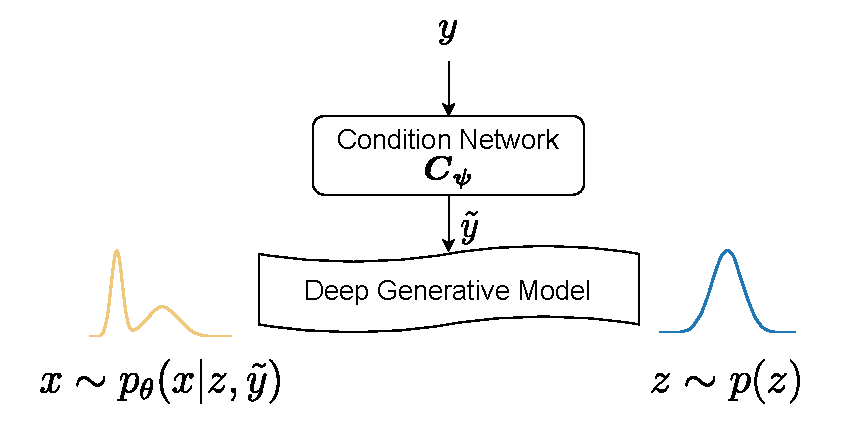
\includegraphics[width=\textwidth, valign=t]{figures/DGM_ABI.pdf}
        \caption[Universal Framework of Using Deep Generative Models for Amortized Bayesian Inference]{\small Universal Framework of Using Deep Generative Models for Amortized Bayesian Inference. The corresponding algorithm is shown on the right (Algorithm \ref{alg:dgm_abi}).}
        \label{fig:universal_framework}
        \vspace{0.5em}
        \small
        \begin{tabular}{@{}p{0.12\linewidth}p{0.4\linewidth}p{0.4\linewidth}@{}}
        \toprule
        \textbf{Model} & \makecell[l]{\textbf{Training}\\\textbf{Objective}} & \textbf{Inference} \\
        \midrule
        VAE & Maximize ELBO & Amortized encoder \\
        NF & \makecell[l]{Maximize\\log-likelihood} & Direct deterministic mapping \\
        FM & Minimize matching cost (vector field) & Integrate ODE \\
        SBM & Minimize matching cost (score function) & Integrate SDE \\
        DDPM & Minimize matching cost (added noise) & Integrate SDE \\
        \bottomrule
        \end{tabular}
        \captionof{table}{Training paradigms and inference across \acp{DGM}.}
        \label{tab:dgm_training_inference}
    \end{minipage}
    \hfill
    \begin{minipage}[t]{0.48\textwidth}
        \vspace{0pt}\vspace{-1.5ex}
        \begin{algorithm}[H]
            \caption{DGM-ABI Training \& Inference}
            \label{alg:dgm_abi}
            \begin{algorithmic}[1]
            \normalsize
            \REQUIRE Dataset $\mathcal{D} = \{(x^{(i)}, y^{(i)})\}_{i=1}^M$
            \REQUIRE Prior $p(z)$, Condition network $C_\psi$
            \REQUIRE Generator $p_\theta(x \mid z, \tilde{y})$, (Optional: Inference $q_\phi(z \mid x, \tilde{y})$)
            
            \vspace{0.1cm}
            \STATE \textbf{Stage 1: Amortized Learning}
            \WHILE{not converged}
                \STATE Sample batch $\{(x, y)\} \sim \mathcal{D}$
                \STATE Compute embeddings: $\tilde{y} \leftarrow C_\psi(y)$
                \STATE Sample latent: $z \sim p(z)$
                \STATE Compute objective gradient:
                \STATE $g \leftarrow \nabla_{\theta,\psi,\phi} \, \mathcal{L}$
                \STATE Update parameters: $(\theta, \psi, \phi) \leftarrow (\theta, \psi, \phi) - \eta \cdot g$
            \ENDWHILE

            \STATE \textbf{Stage 2: Bayesian Inference}
            \STATE Given observed condition $y_{\text{obs}}$:
            \STATE $\tilde{y}_{\text{obs}} \leftarrow C_\psi(y_{\text{obs}})$
            \FOR{$k=1$ to $K$}
                \STATE Sample $z^{(k)} \sim p(z)$
                \STATE Generate $x^{(k)} \sim p_\theta(x \mid z^{(k)}, \tilde{y}_{\text{obs}})$
            \ENDFOR
            \RETURN Posterior samples $\{x^{(k)}\}_{k=1}^K$
            \end{algorithmic}
        \end{algorithm}
    \end{minipage}
\end{figure}

\subsection{Normalizing Flows for Parameter Identification}
Why are \acp{NF} more suitable for parameter identification tasks given time series observations? In this section, we will answer this question in terms of (1) inference accuracy and precision, (2) reliability, i.e., whether the ground truth lies in the posterior, (3) speed, i.e., inference computational time, (4) sample efficiency, i.e., posterior contraction while increasing data amount, (5) correlation, i.e., identifying linearly correlated parameters, (6) complexity, i.e., handling multimodal distributions.

\subsubsection{Overall Settings}
In this section, we take a classic mass-spring-damper system as an example, which has three parameters including mass $m$, spring constant $k$, and damping coefficient $c$. As observations, we take the position and velocity trajectories. For evaluation of (1) - (4), an external force is introduced. The \ac{ODE} is:
\begin{equation}
    \dot x = v,\; \dot v = \frac{1}{m}(F_t-kx-cv),\; F_t = 10\cdot \sin(3t).
\end{equation}

For the (5) linear correlation case, the external force is removed, and the parameters $m$ and $k$ are correlated, i.e., $k=10\cdot m$. To investigate the (6) multimodal case, the system is extended into the topology Wall -- $k_1$ -- $m$ -- $k_2$ -- $m$ -- $k_3$ -- Wall. When the parameters $m$, $k_2$, and $c$ are fixed as constant, and we take the middle points of the positions and velocities of the two masses as observations, the value of $k_1$ and $k_3$ cannot be uniquely distinguished. The \ac{ODE} becomes
\begin{align}
    \dot x_1 &= v_1,\;\dot v_1=\frac{1}{m}(-k_1x_1+k_2(x_2-x_1)-cv_1);\\
    \dot x_2 &= v_2,\;\dot v_2=\frac{1}{m}(-k_3x_2-k_2(x_2-x_1)-cv_2).
\end{align}

We compare two normalizing flow architectures \ac{RealNVP} and \ac{NSF} with \ac{FM}, \ac{DDPM}, and \ac{SBM}, as well as \ac{VAE} and \ac{BNN}. As the condition network, we use an \ac{LSTM} layer followed by two linear layers with \ac{ELU} activations. For a group of estimated $\{ \widehat{x}^{(m)}\}_{m=1}^{M}$ and true parameters $ \{ x^{(m)}\}_{m=1}^{M}$ with the mean of the true parameters $\overline{x}$, the following evaluation metrics are applied:
\begin{itemize}
    \item Accuracy: \ac{RMSE} and R² score:
    \begin{equation}
        RMSE = \sqrt{\frac{1}{M}\sum_{m=1}^M (x^{(m)} - \widehat{x}^{(m)})^2}\;,
    \end{equation}
    \begin{equation}
        R^2 = 1 - \sum_{m=1}^{M}\frac{(x^{(m)}-\widehat{x}^{(m)})^2}{(x^{(m)}-\overline{x})^2}\;.
    \end{equation}

    \item Precision: \ac{MCIW}. For the $m$-th parameter by sampling it $L$ times, the standard deviation is $\sigma_{\widehat{x}^{(m)}}$, and we have:
    \begin{equation}
        CI^{(m)}(95\,\%)= [L_{m}, U_{m}] = \widehat{x}^{(m)}\pm 1.96\frac{\sigma_{\widehat{x}^{(m)}}}{\sqrt{L}}.
    \end{equation}
    Then the MCIW can be obtained by:
    \begin{equation}
        MCIW = \frac{1}{M}\sum_{m=1}^{M}(U_m - L_m).
    \end{equation}
    \item Reliability: \ac{CICP}. The larger \ac{CICP} indicates higher reliability of estimation.
    \begin{equation}
        CICP = \frac{1}{M}\sum_{m=1}^{M}c_m, \:
        c_m  = \begin{cases}
                0 & \text{ if } x ^{(m)} \notin [L_{m}, U_{m}], \\ 
                1 & \text{ otherwise. } 
              \end{cases}
    \end{equation}
\end{itemize}

\subsubsection{Performance Comparison (Winner: RealNVP)}
\begin{table}[ht]
    \centering
    \caption[Performance Benchmarking of Deep Bayesian Inference Methods]{Performance Benchmarking of Deep Bayesian Inference Methods on the Mass-Spring-Damper System. All metrics represent averages across the three system parameters. Predictive accuracy is assessed via RMSE (lower is better) and R² (higher is better). Uncertainty quantification is evaluated through the CICP and MCIW together. Ideal performance is characterized by a CICP near the 95\,\% calibration target; significantly lower values indicate overconfidence, while excessively high MCIW values indicate model imprecision. Inference time denotes the total computational time for a single test scenario based on \num{100} posterior samples.}
    \label{tab:metrics_005}
    \small
    \begin{tabular}{lccccc}
        \toprule
        \textbf{Model} & \textbf{RMSE} $\downarrow$ & \textbf{$R^2$} $\uparrow$ & \textbf{CICP} $\uparrow$ & \textbf{MCIW} $\downarrow$ & \textbf{Inference Time (\si{s})} $\downarrow$ \\ 
        \midrule
        BNN     & 0.0393 & 0.9965 & 0.9900 & 0.1874 & 0.0209 \\
        VAE     & 0.0287 & \textbf{0.9987} & 0.7250 & \textbf{0.0497} & \textbf{0.0018} \\
        DDPM    & 0.0915 & 0.9852 & 0.9883 & 0.5338 & 0.2310 \\
        SBM     & 0.0699 & 0.9909 & 0.9700 & 0.3289 & 0.0534 \\
        FM      & 0.0547 & 0.9938 & \textbf{0.9933} & 0.3730 & 0.0050 \\
        RealNVP & \textbf{0.0278} & 0.9986 & 0.9917 & 0.1223 & 0.0043 \\
        NSF     & 0.0401 & 0.9966 & 0.9917 & 0.1845 & 0.0069 \\
        \bottomrule
    \end{tabular}
\end{table}

\begin{figure}[htp!]
    \begin{minipage}{0.7\textwidth}
        \centering
        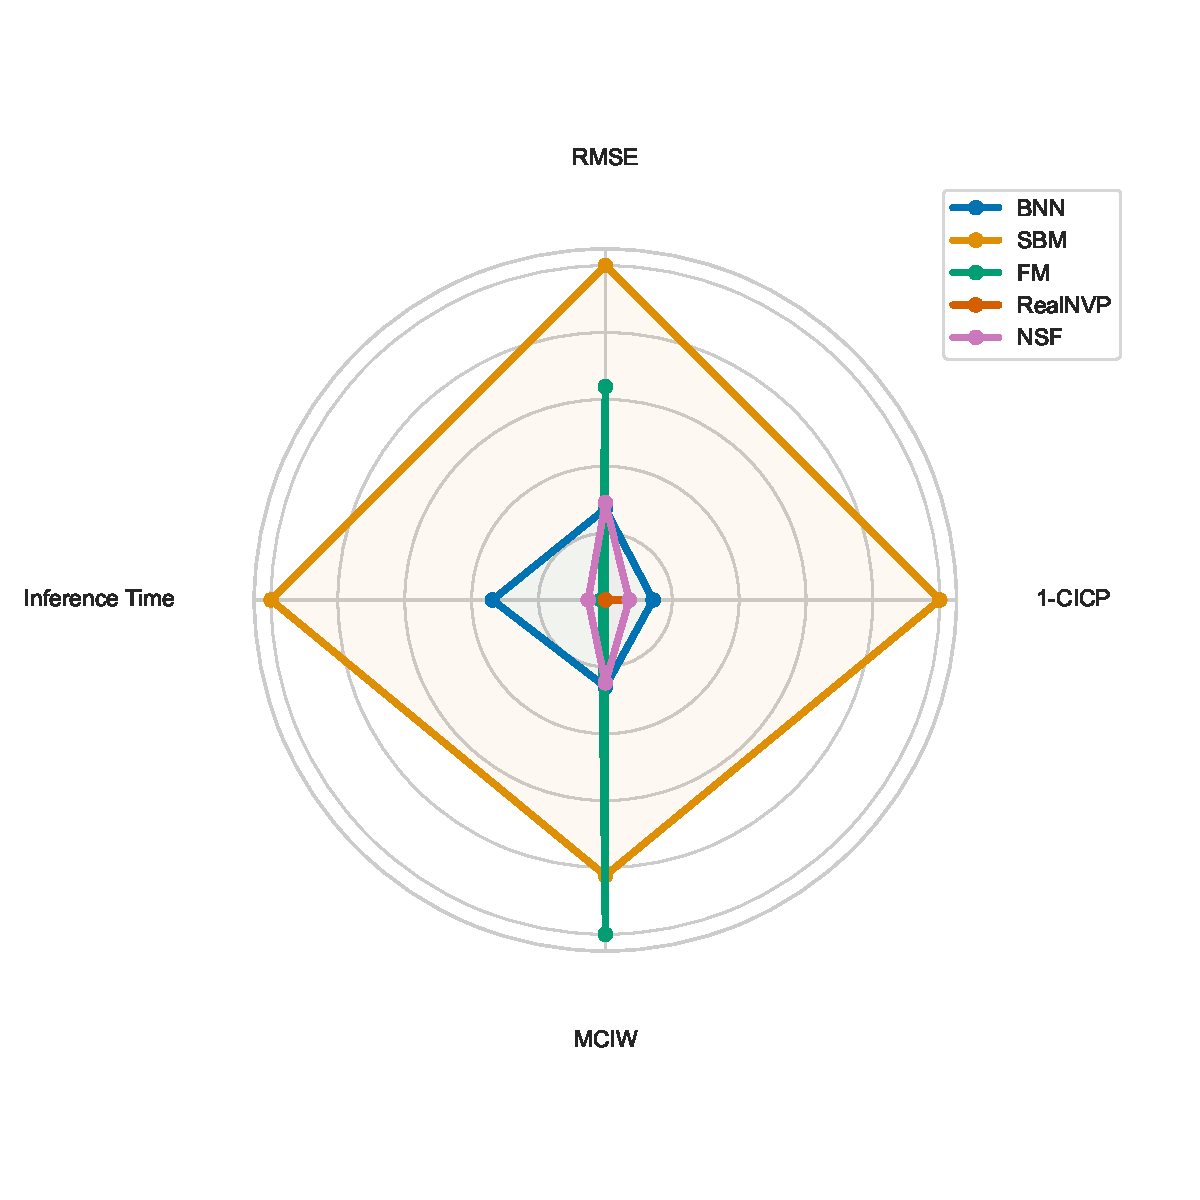
\includegraphics [width=\linewidth, trim=0 50pt 0 50pt, clip]{figures/metrics_0.05_spider_chart.pdf}
      \end{minipage}
      \hfill
    \begin{minipage}{0.28\textwidth}
    \caption[Detailed Comparison of Deep Bayesian Inference Methods]{Detailed Comparison of Deep Bayesian Inference Methods on the Mass-Spring-Damper System. The values are the same as those in Table~\ref{tab:metrics_005}. 1-CICP is shown for the sake of consistency of comparison, meaning that for all metrics in the spider chart, lower is better. The center of the radar plot represents optimal performance.}
    \label{fig:metrics_005_spider}
    \end{minipage}
\end{figure}

In Table~\ref{tab:metrics_005}, the evaluation of different models is shown. The observed time series are from \SI{0}{s} to \SI{1}{s} with the time step of \SI{0.05}{s}, and no noises are added onto them. In terms of accuracy, \ac{RealNVP} (RMSE: 0.0278) and VAE (RMSE: 0.0287) are the most accurate models. Their highest R² scores indicate that they explain almost all the variance in the mass-spring-damper system. \ac{DDPM} (RMSE: 0.0915) has the highest error in this group. While an R² of 0.985 is still objectively good, it is significantly less precise than the \acp{NF} (\ac{RealNVP}, \ac{NSF}) for this specific physical task. Overall, the flow-based methods (\ac{RealNVP}, \ac{NSF}, and \ac{FM}) achieve higher accuracy than diffusion-based methods (\ac{DDPM} and \ac{SBM}). The \ac{BNN} is comparable with the \acp{NF}.

In terms of uncertainty quantification, almost all models (except VAE) show CICP values near 1.0. Theoretically, the ideal CICP with 95\,\% confidence intervals should also be 0.95. Higher CICPs mean that they are conservative and under-confident, whereas the lower CICPs indicate overfitting. Besides, in an ideal noise-free scenario, the posterior distribution for the mass-spring-damper parameters should approach a Dirac delta function. However, in the practice of solving inverse problems, the interval should never be zero, because different parameters might produce very similar trajectories. Moreover, the models themselves have uncertainty due to limited data. Therefore, the CICPs higher than 0.95 mean that the inference models prioritize the reliability over precision.  Consequently, the MCIW should be considered together with CICP. \ac{VAE} (CICP: 0.7250 and MCIW: 0.0497) is overconfident. Its intervals are so narrow that the truth falls outside of them 27.5\,\% of the cases. \ac{DDPM} (CICP: 0.9883 and MCIW: 0.5338) is imprecise. It achieves high coverage simply by producing very wide intervals. 

In terms of computational efficiency, \ac{VAE} exhibits the highest inference speed. Flow-based methods demonstrate comparable performance to one another, though they are approximately $5\times$ slower than the \ac{VAE} baseline. \ac{BNN} follows, showing higher latency than the flow-based models but maintaining a clear advantage over \ac{SBM}. Finally, \ac{DDPM} is identified as the most computationally intensive approach, recording the slowest inference times.

With \ac{VAE} and \ac{DDPM} excluded due to miscalibration and computational overhead respectively, Figure~\ref{fig:metrics_005_spider} visualizes the performance trade-offs of the remaining five architectures. \ac{RealNVP} exhibits the most optimal profile, represented by the smallest polygon area; it successfully minimizes \ac{RMSE} and \ac{MCIW} while maintaining near-perfect coverage. \ac{NSF} and \ac{FM} show comparable speed and accuracy but yield less precise (wider) credible intervals. The \ac{BNN} maintains high reliability (low 1-CICP) but suffers from increased inference time. Finally, \ac{SBM} shows the least favorable performance, characterized by the largest predictive error, the widest uncertainty bounds, and the longest computational time, indicating a difficulty in parameter identification compared to flow-based alternatives. 

\subsubsection{Sample Efficiency (Winner: RealNVP)}
\begin{figure}[htp!]
    \centering
    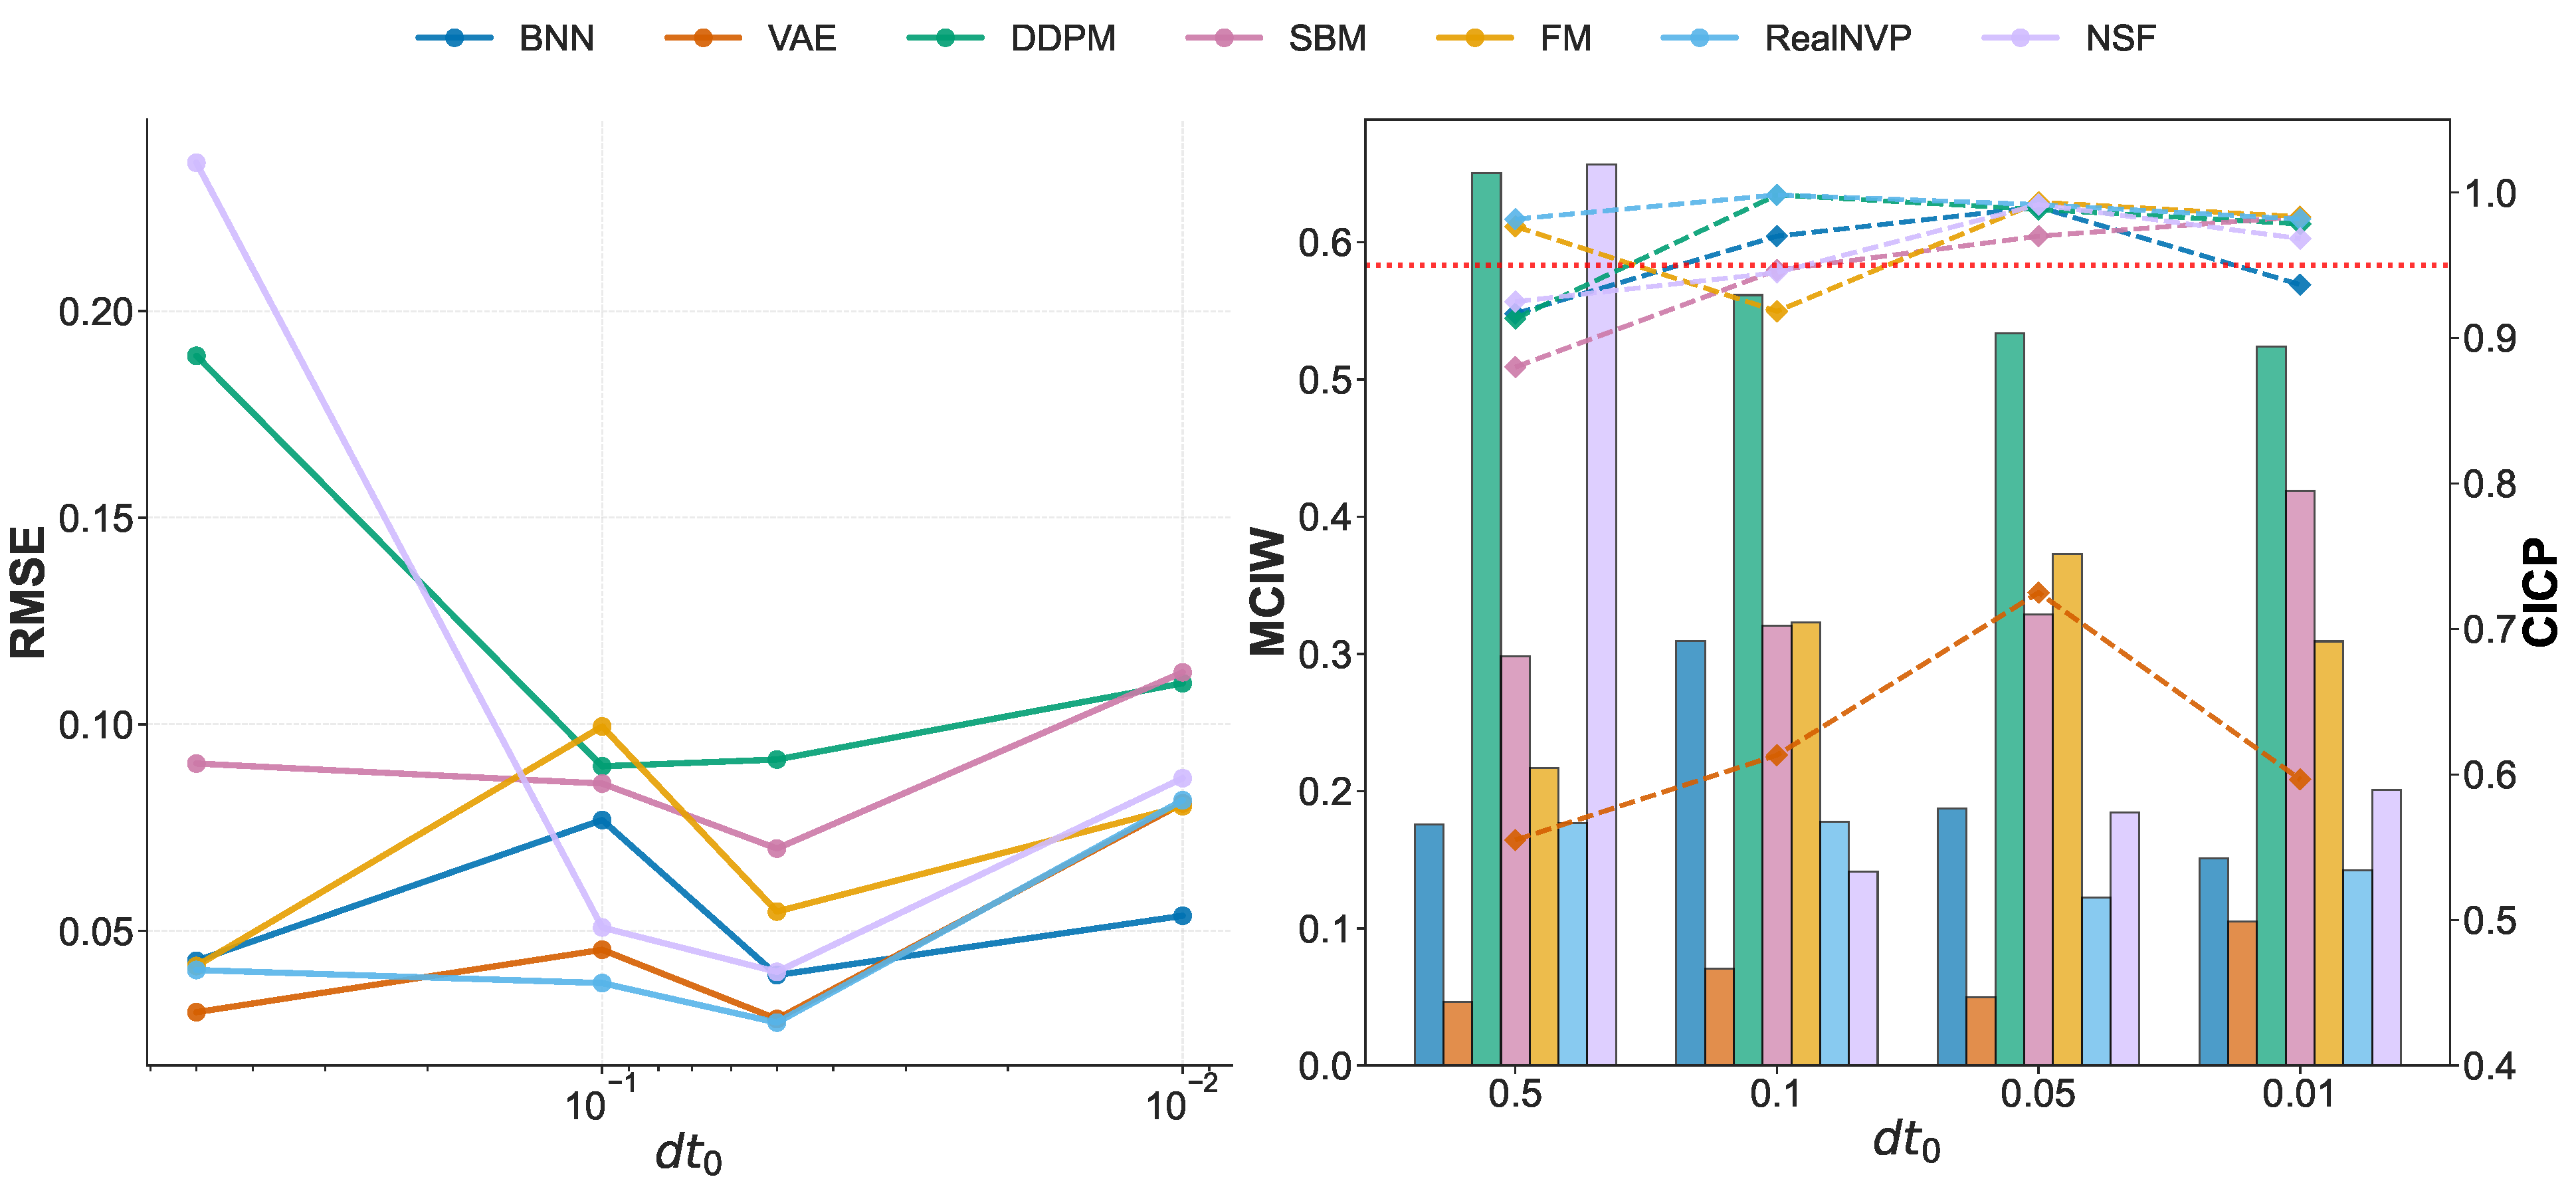
\includegraphics[width=\textwidth]{figures/curve_chart_sample.pdf}
    \caption[Performance Comparison w.r.t. Sample Efficiency]{Sample Efficiency Comparison of Deep Bayesian Inference Methods under Varying Observation Densities. The left panel illustrates the predictive accuracy (RMSE) across time step $dt_0=[\SIlist{0.5;0.1;0.05;0.01}{s}]$ plotted on a logarithmic scale where smaller $dt_0$ represents higher sampling density. The right panel provides a hybrid uncertainty analysis: the grouped bars indicate the MCIW (uncertainty precision), while the superimposed dashed lines represent the CICP (calibration reliability). The horizontal dotted line denotes the 95\,\% coverage target.}
    \label{fig:se_comp}
\end{figure}

Figure~\ref{fig:se_comp} shows how observation density affects posterior estimation. As $dt_0$ decreases from \SI{0.5}{s} to \SI{0.05}{s}, all models show consistent improvement in predictive accuracy, attributed to improved identifiability of the system dynamics. Accuracy degrades at $dt_0=\SI{0.01}{s}$---likely because the encoder is not designed for long time series. Adding more points adds redundancy without new constraints; this can induce overfitting in the latent space, where the model interprets numerical rounding errors or minor architectural biases as significant physical features. For this system, \SI{0.05}{s} is the optimal resolution. \ac{BNN}, \ac{RealNVP}, and \ac{VAE} are less sensitive to sample efficiency; diffusion-based methods and \ac{NSF} require more data. While almost all models reach their accuracy peak at $dt_0=\SI{0.05}{s}$, \ac{FM} favors lower resolution, possibly because vector-field learning benefits from larger differences between data samples.

Regarding uncertainty quantification, \ac{VAE} is overfitted with narrow intervals and inadequate coverage. As data density increases, \ac{DDPM} and \ac{RealNVP} show consistent posterior shrinkage---as the likelihood becomes more peaked, the posterior contracts around the true parameters. Other architectures exhibit more volatile trends: the MCIW of \ac{BNN} initially increases before dropping; \ac{NSF} shows a decrease-then-rise pattern; \ac{FM} and \ac{SBM} show paradoxical MCIW increases, as the longer sequences introduce numerical complexity or perceived contradictions in the latent space that temporarily outweigh the additional information. The reliability requirement (\ac{CICP} $\ge 0.95$) is hardest under sparse sampling. At $dt_0=\SI{0.5}{s}$, only \ac{RealNVP} and \ac{FM} are calibrated, highlighting their robustness for sparse trajectories. As density improves to $dt_0=\SI{0.1}{s}$, \ac{FM} temporarily drops out of the reliable regime (its MCIW rise not aligned with predictive accuracy), while \ac{SBM} and \ac{NSF} reach the target via distinct mechanisms---\ac{SBM} through corrective expansion of posterior variance, \ac{NSF} through efficient shrinkage. At $dt_0=\SI{0.05}{s}$, all models satisfy the requirement; \SI{0.05}{s} provides sufficient information without numerical saturation.

At the highest density ($dt_0=\SI{0.01}{s}$), models break down. \ac{DDPM} and \ac{BNN} continue to shrink MCIW; for \ac{BNN}, intervals shrink faster than error, causing it to miss the ground truth and become overconfident. Conversely, \ac{SBM}, \ac{RealNVP}, and \ac{NSF} expand MCIW defensively, as the numerical difficulty of processing high-frequency noise-free data broadens uncertainty bounds to maintain coverage. \ac{FM} reverses its trend and eventually finds a more stable numerical representation than the other flow variants. In summary, more observations do not always improve performance. \ac{RealNVP} is most precise under sparse data (excluding \ac{VAE}); \ac{BNN} shrinks bounds consistently but its variance may reflect weight convergence rather than physical correctness. Notably, at $dt_0=\SI{0.1}{s}$, \ac{SBM} and \ac{NSF} define the boundary of the reliable regime, whereas \ac{BNN} and \ac{DDPM} remain under-calibrated despite increased data density.

\subsubsection{Linear Correlation (Winners: SBM, RealNVP, NSF)}
When parameters are linearly correlated, the observations only constrain their ratio, rendering the individual parameters non-identifiable. While \acp{DGM} are capable of capturing these dependencies, the task is computationally harder than identifiable ones. The ill-posedness manifests as a manifold of equivalent solutions, making it difficult for optimization algorithms to distinguish between physically distinct systems that produce identical observations. When the correlation between $m$ and $k$ are fixed to be $k=10\cdot m$, the damping coefficient should also be proportional to the mass, i.e., $c\propto m$. The damping coefficient $c$ is related to the damping ratio $\zeta$ (which determines if the system is under-damped, critically damped, or over-damped) by the formula:
\begin{equation}
    c=2\zeta\sqrt{mk}.
\end{equation} 
Therefore, the following relation holds:
\begin{equation}
    c/m = 2\sqrt{10}\;\zeta.
\end{equation}
Figure~\ref{fig:lc_comp} shows two identification examples of linear correlated parameters.
\begin{figure}[htp!]
    \centering
    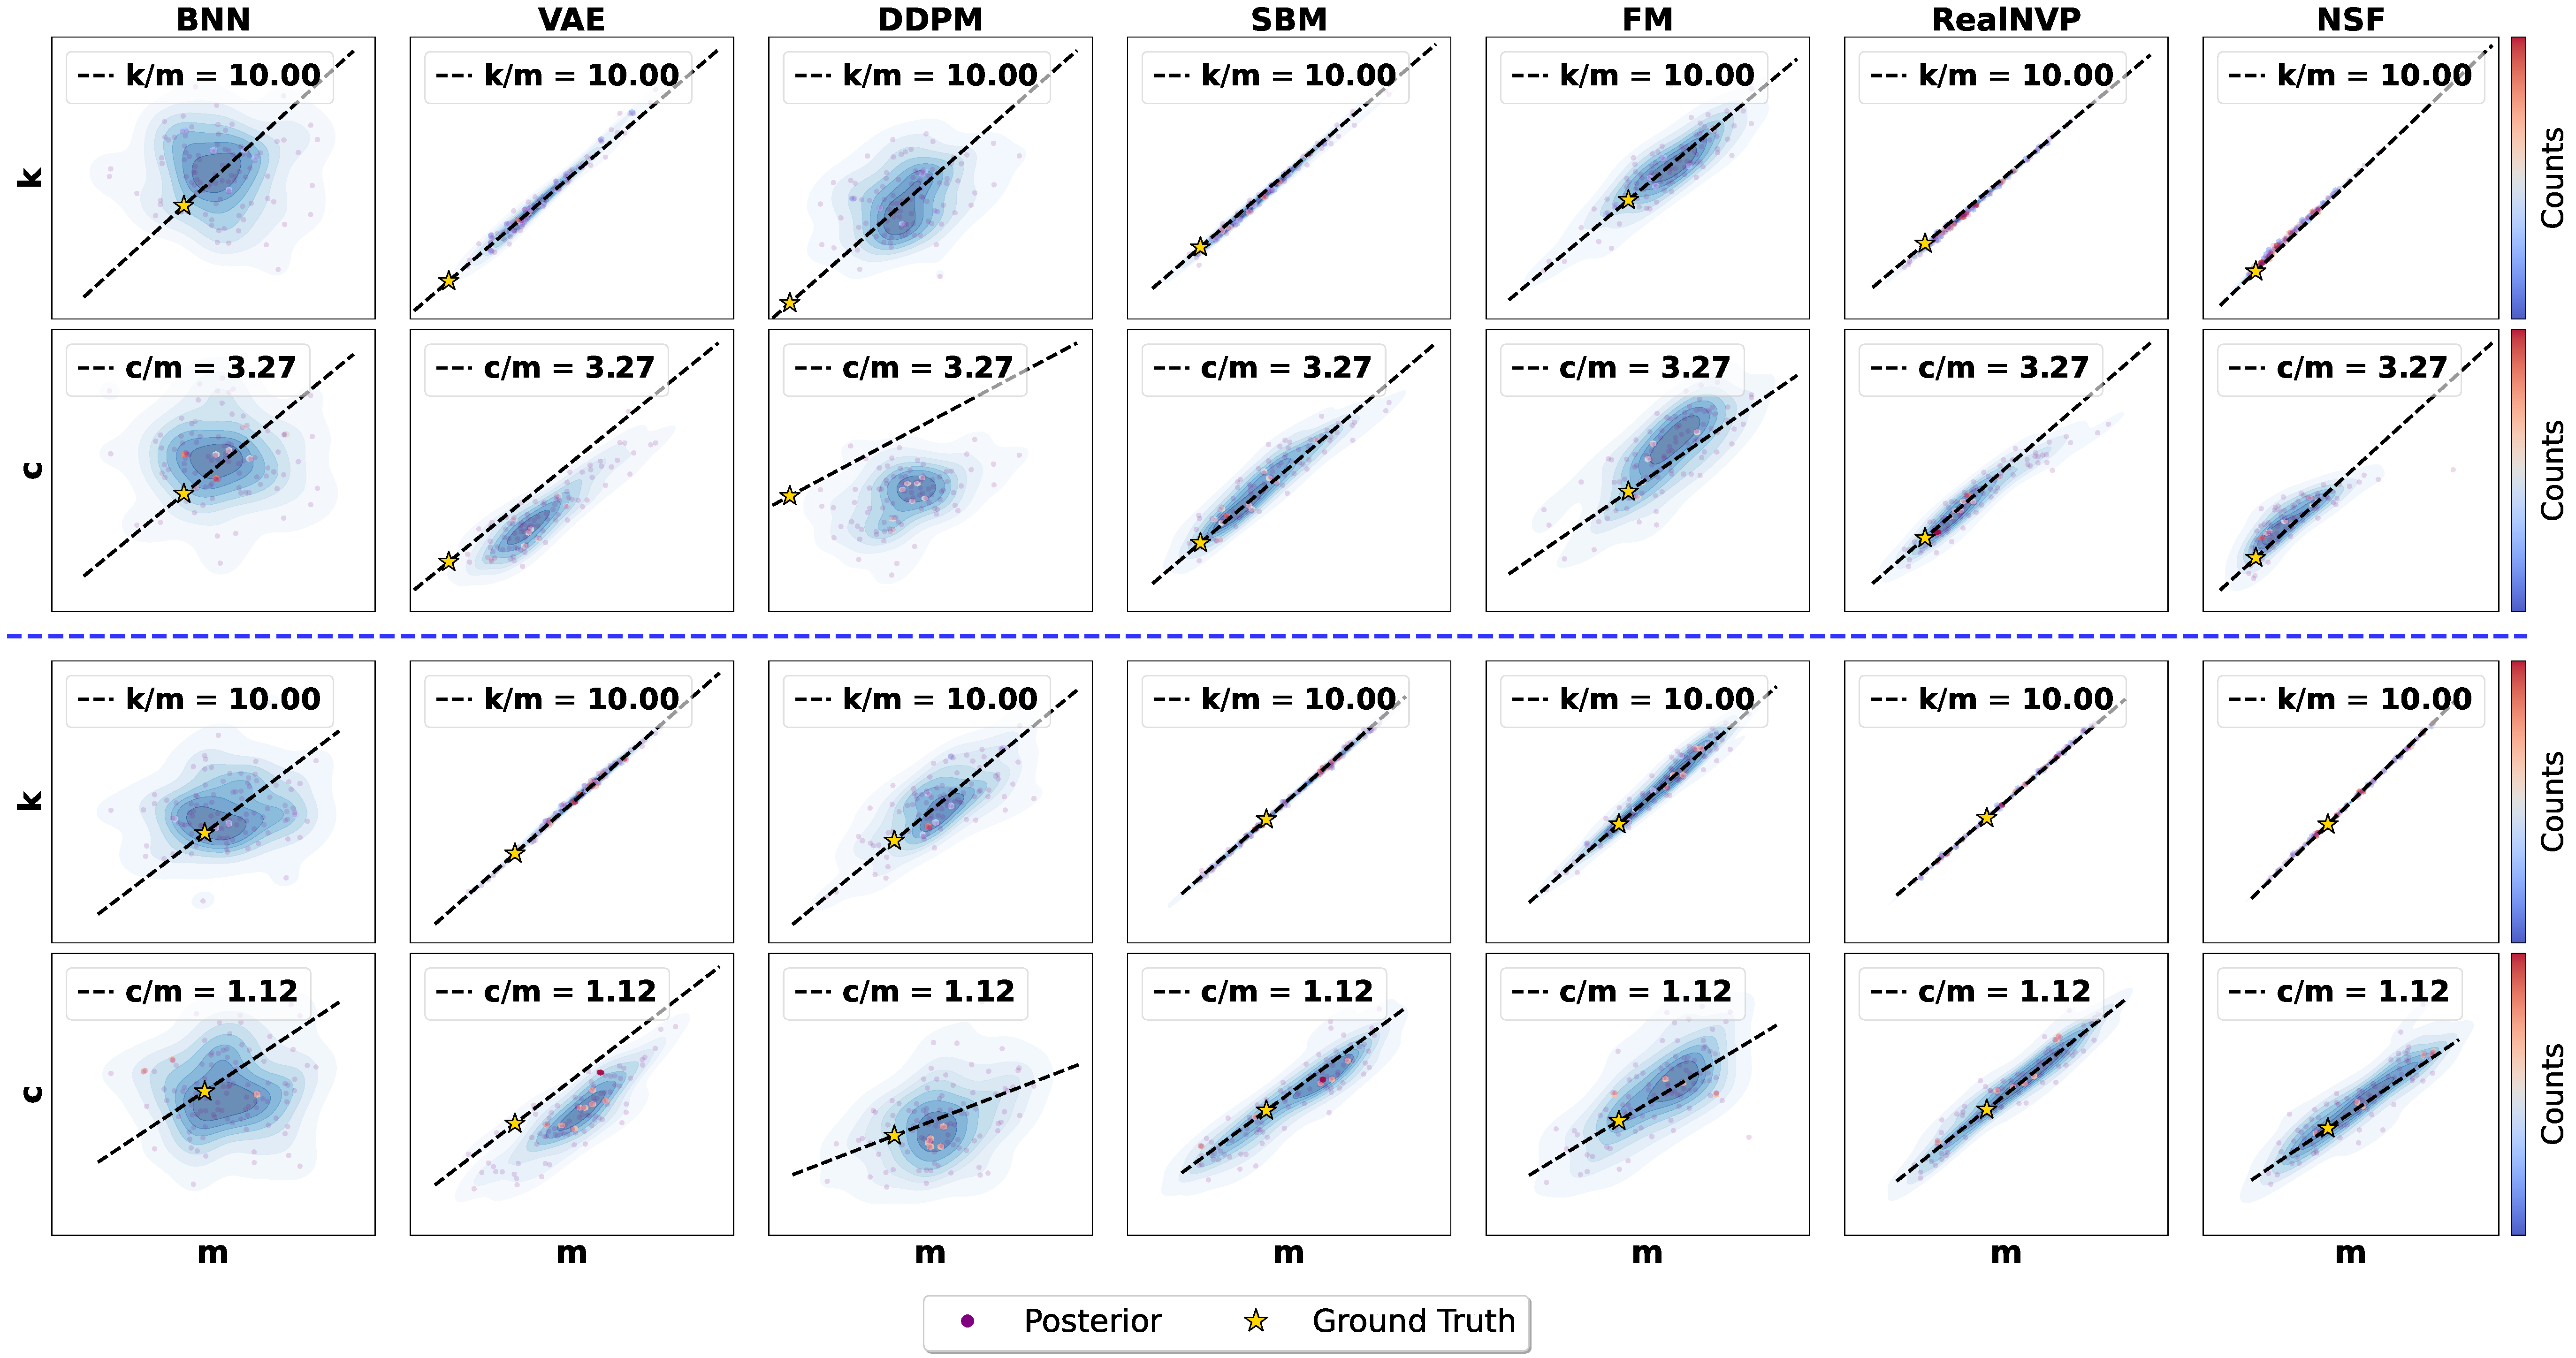
\includegraphics[width=\textwidth]{figures/model_comparison_grid_linear.pdf}
    \caption[Linear Correlation Comparison]{Comparative analysis of deep Bayesian inference architectures in identifying linearly correlated parameters. The $4\times7$ grid displays the joint posterior distributions for seven different models (columns) across two test scenarios (separated by a horizontal blue dashed line in the middle). Rows 1 and 3 visualize the $m-k$ correlation, while Rows 2 and 4 visualize the $m-c$ correlation. Within each sub-figure, the gold star represents the ground truth, and the black dashed line illustrates the theoretical linear constraint ($k/m$ or $c/m$). Individual posterior samples are plotted as purple points, overlaid on a logarithmic density heatmap where warm hues indicate regions of high probability mass. Note: To ensure high visibility of the posterior topology across models with varying precision, axis limits and density color-scales are individually optimized for each sub-figure. Each color map suits the whole row.}
    \label{fig:lc_comp}
\end{figure}

As illustrated in Figure~\ref{fig:lc_comp}, the \ac{BNN} and \ac{DDPM} fail to capture the underlying dependencies, resulting in wide, uninformative posterior clouds that lack alignment with the physical constraints. While the \ac{VAE} recovers the $k/m$ correlation, it fails significantly on $c/m$, where the posterior mass is biased and poorly aligned with the diagonal line. In contrast, the remaining four methods demonstrate higher fidelity. 

Among the successful models, \ac{SBM} and the \ac{NF} architectures (\ac{RealNVP} and \ac{NSF}) show their superior capability in identifying and enforcing linear parameter correlations. Their $k/m$ estimates are tightly aligned with the theoretical diagonal, and their $c/m$ estimates manifest as narrow ellipses centered on the ground truth. On the other hand, \ac{FM} successfully captures the linear trend, but it exhibits noticeably higher variance compared to \ac{SBM}, \ac{RealNVP}, and \ac{NSF}, particularly in the $c/m$ correlations. This suggests that while \ac{FM} identifies the correlation, it is less precise in enforcing the constraint than other architectures.

Linear correlations represent a low-dimensional manifold within the parameter space. Figure~\ref{fig:lc_comp} demonstrates that \acp{NF} (\ac{RealNVP}/\ac{NSF}) and \ac{SBM} are superior at manifold learning by effectively collapsing the posterior mass onto a line, whereas \ac{BNN} and \ac{DDPM} struggle to resolve such sharp constraints. Besides, the \ac{VAE}’s failure in the $c/m$ correlation is a classic symptom of posterior collapse or architectural under-fitting for specific parameter dimensions. 

The performance gap between the two diffusion models is particularly striking: \ac{SBM} exhibits a far greater capability for recovering precise physical constraints than \ac{DDPM}. Despite \ac{DDPM}'s established success in generating high-dimensional complex data, it fails to resolve the specific linear parameter correlations in this task.
Similarly, despite their theoretical proximity, \ac{FM} appears more dispersed than \ac{SBM}. This is primarily because \ac{FM} is a deterministic transport method that is more sensitive to cumulative approximation errors along the integration path, whereas the stochastic nature of \ac{SBM} provides a corrective mechanism through noise-driven sampling.

Within the \ac{NF} architectures, a notable distinction exists between \ac{RealNVP} and \ac{NSF} when we zoom in on the $c/m$ figures. While both successfully identify the correlation, \ac{RealNVP} exhibits a higher degree of centralization along the diagonal correlation axes. While this leads to a narrower, line-like distribution with high precision, it also places the ground-truth (yellow star) at the extreme periphery of the high-density core. In contrast, \ac{NSF} estimates the density with higher variance, which is less desirable in this case. 

\begin{figure}[H]
    \centering
    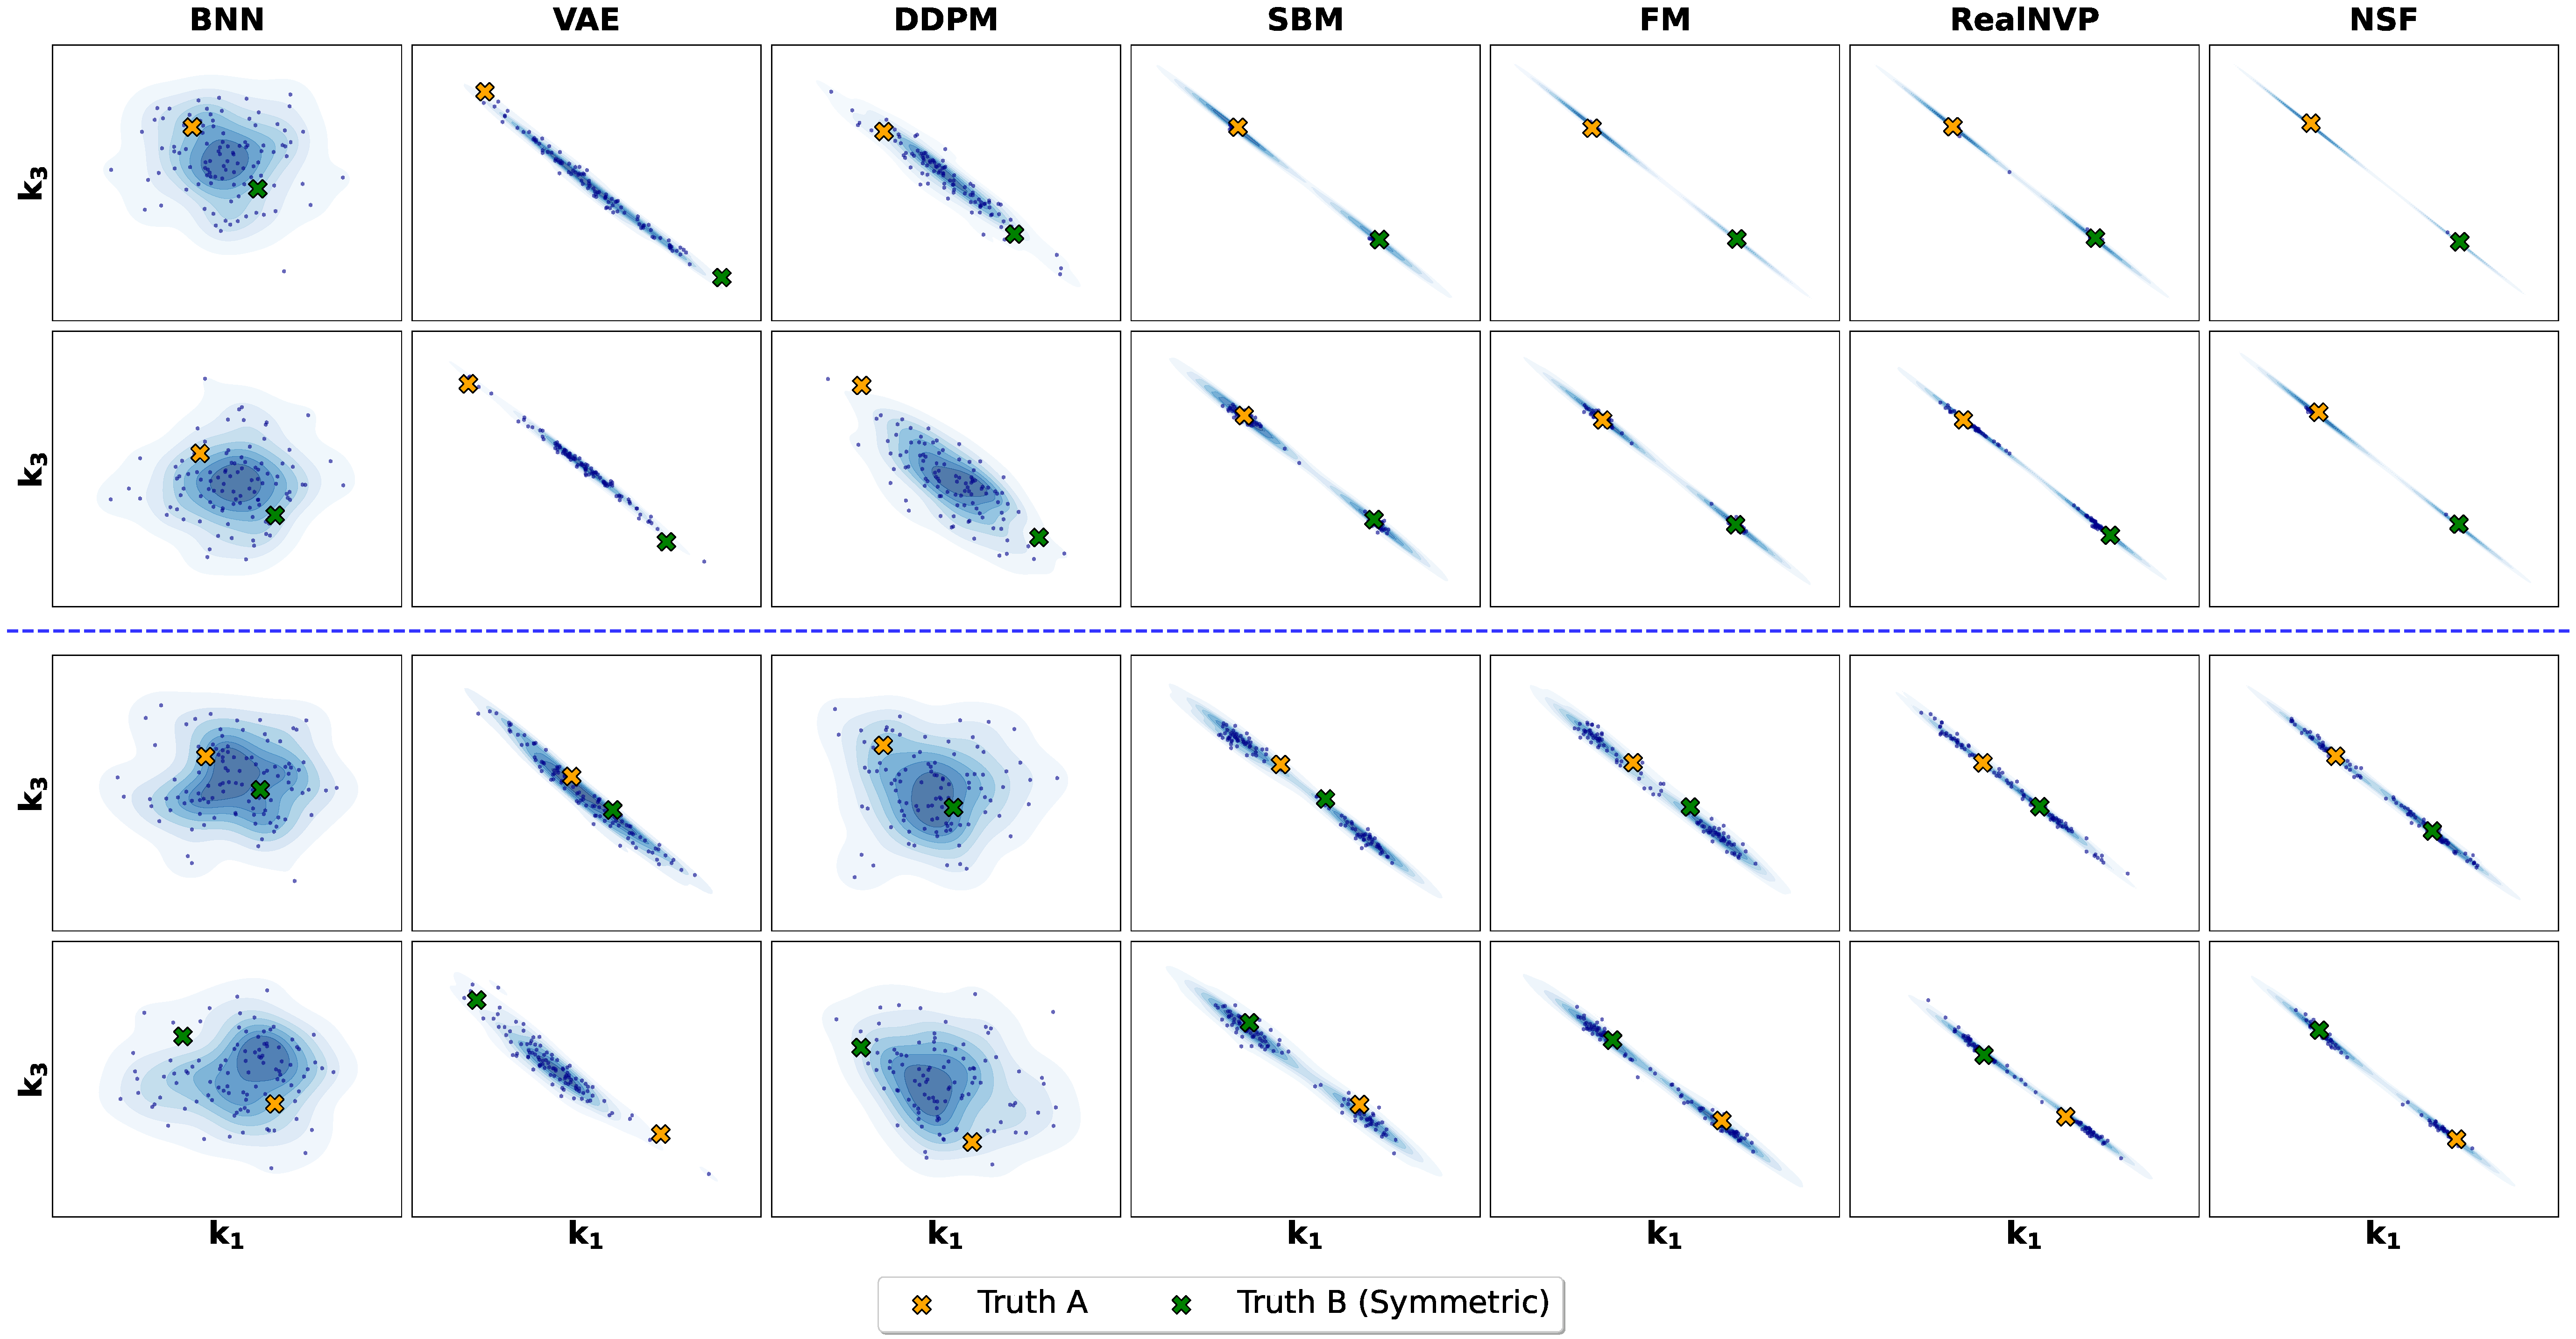
\includegraphics[width=\textwidth]{figures/model_comparison_grid_multi_modal.pdf}
    \caption[Multimodal Comparison]{Comparative evaluation of deep Bayesian architectures in recovering multimodal posterior distributions. The $4\times7$ grid displays the joint posterior of $k_1$ and $k_3$ for seven different models (columns) across four distinct test scenarios (rows). The top two rows represent scenarios with well-separated modes, while the bottom two rows represent scenarios with proximal (overlapping) modes (partitioned by a blue dashed line). Within each subplot, the orange cross denotes the target ground truth, while the green cross represents the symmetric ground truth (swapped $k_1$ and $k_3$ values), highlighting the models' ability to capture the inherent exchangeable symmetry of the parameter space. Blue contours represent the estimated posterior density. Note: To ensure high visibility of the posterior topology across models with varying precision, axis limits and density color-scales are individually optimized for each sub-figure.}
    \label{fig:mm_comp}
\end{figure}

\subsubsection{Multimodal Distribution (Winner: NSF)}
The ability to capture multimodal distributions is a key advantage of applying \acp{DGM} for Bayesian inference. Different \acp{DGM} exhibit different characteristics. Figure~\ref{fig:mm_comp} illustrates these differences. As test scenarios, we consider two cases: one where the values of $k_1$ and $k_3$ are far apart (the first two samples), and another where they are close to each other (the last two samples).
 
As demonstrated in Figure~\ref{fig:mm_comp}, the performance is consistent with the linear correlation results. \ac{SBM}, \ac{FM}, \ac{NSF}, and \ac{RealNVP} significantly outperform \ac{BNN}, \ac{VAE}, and \ac{DDPM} in resolving the symmetric multimodal structure.
The \ac{BNN} produces broad, uninformative posterior clouds that fail to recognize any specific multimodal topology. The \ac{VAE} exhibits over-concentration onto narrow, biased ridges; in all these four scenarios, the ground truth and its symmetric counterpart lie entirely outside the high-density regions, indicating the posterior collapse again. \ac{DDPM} successfully resolves the two distinct modes only in the first scenario (Row 1), but degrades into a single diffuse, biased cluster in the remaining test cases.

In contrast, \ac{SBM} and the three \ac{NF} architectures (\ac{RealNVP}, \ac{NSF}, and \ac{FM}) demonstrate a superior capacity for multimodal recovery. In well-separated scenarios (top two rows), all architectures successfully resolve two distinct high-probability modes. Notably, however, \ac{RealNVP} exhibits a slight bias, failing to precisely align its right posterior mode with the ground truth. As the modes become proximal (bottom two rows), the identification task becomes increasingly ill-posed, with models struggling to decouple the two ground-truth points and producing a higher density of samples in the interstitial region. While \ac{NSF} maintains high fidelity by successfully resolving both modes and accurately centering the posterior on the ground-truth coordinates, the remaining three models exhibit varying degrees of dislocation. This suggests that while most architectures can handle discrete multimodality, only \ac{NSF} remains robust in proximal scenarios where structural symmetry leads to significant parametric overlap.

\subsection{Relationship Between Bayesian Inference and Sensitivity Analysis}
Previous experiments applying mass-spring-damper models demonstrate that Bayesian inference is intrinsically linked to parameter identifiability. Our findings indicate that spring constants converge rapidly during training, which will be further elucidated through sensitivity analysis. Conversely, linearly correlated parameters lack unique identification, and in symmetric coupled models, individual spring constants become indistinguishable. These varying levels of identifiability can be rigorously analyzed through \ac{SA}, which studies how uncertainty in the output of a mathematical model can be partitioned and allocated to different sources of uncertainty in its inputs. This framework aligns naturally with the objectives of amortized Bayesian inference. For purely data-driven methods, \ac{SA} provides essential insights into the physical model and practical training suggestions: weakly identifiable or correlated parameters that require additional observational data for resolution.

Unlike local \ac{SA}, which examines instantaneous changes in output relative to specific parameter perturbations, our research focuses on total trajectories, necessitating a global \ac{SA}. 

\subsubsection{Sobol' index}
A common approach for global \ac{SA} is the Sobol' index, which is a variance-based method that decomposes the total output variance into contributions from individual parameters and their interactions. For a model $f$ with inputs $X_1, \ldots, X_d$ and the output $Y$, the total variance of the model output is:
\begin{equation}
    Var(Y) = \sum_i V_i + \sum_{i<j} V_{ij} + \cdots + V_{1,2,\ldots,d}.
\end{equation}
The first-order Sobol' index $S^1_i$ measures the contribution of a single parameter $X_i$ to the output variance, which can be regarded as the main effect. It is given by:
\begin{equation}
    S^1_i = \frac{V_i}{Var(Y)},\quad V_i=Var_{X_i}[E_{\boldsymbol{X}_{\backslash i}}(Y|X_i)].
\end{equation}
The total Sobol' index accounts for the total contribution of a parameter to the output variance, including both its main effect and all higher-order interactions with other parameters. The total Sobol' index of $X_i$ is
\begin{equation}
    S^T_i = \frac{Var_{\boldsymbol{X}_{\backslash i}}[E_{X_i}(Y|\boldsymbol{X}_{\backslash i})]+\sigma_n^2}{Var(Y)+\sigma_n^2}>\frac{Var_{\boldsymbol{X}_{\backslash i}}[E_{X_i}(Y|\boldsymbol{X}_{\backslash i})]}{Var(Y)} > \frac{Var_{\boldsymbol{X}_{\backslash i}}[E_{X_i}(Y|\boldsymbol{X}_{\backslash i})]}{Var(Y)}.
\end{equation}

Another key issue of using variance-based \ac{SA} is to sample the parameter space efficiently. The standard random sampling often creates clusters or gaps in the parameter space. Instead, Sobol' sequences are applied, which are low-discrepancy sequences. For the sake of stability, a larger number of samples should be set.

By comparing these two indices, we can diagnose the structural complexity of the mass-spring-damper system. For instance, a parameter with a high total Sobol' index but a low first-order Sobol' index indicates that while the parameter is influential, its effect is primarily driven by interactions with other components of the model. The linear correlation and multimodality cases are supposed to have zero first-order Sobol' indices and total Sobol' indices of one. 
If a parameter exhibits a total Sobol' index near zero, it suggests that the model output is insensitive to that parameter across its entire prior range. Such parameters are unidentifiable under the provided observed data. 

Ultimately, integrating global \ac{SA} into the amortized Bayesian workflow allows us to preventively identify blind spots in the model. By detecting parameters with low sensitivity or high correlation, we can strategically focus on data collection efforts or reparameterize the model to ensure that the posterior distributions are well-defined and physically meaningful. When parameters exhibit significantly different levels of identifiability, a sensitivity-guided iterative identification strategy is recommended. In such cases, strongly identifiable parameters (those with high $S^1_i$ values, like the primary spring constants) should be identified first to stabilize the model. Once these dominant parameters are constrained, the remaining weakly identifiable or highly correlated parameters can be addressed in subsequent stages by adaptation of observational data or by refining the prior distributions. This hierarchical approach prevents the variance of dominant parameters from obscuring the signals of secondary parameters, ensuring a more robust and physically meaningful calibration of the complex system.

The sensitivity of parameters also reflects the convergence speed of training deep Bayesian inference models as well. Taking a closer look at the mass-spring-damper model with external force, we get very close first-order and total-order indices, i.e., $S^1_m=0.07, S^1_k=0.88, S^1_c=0.03$ and $S^T_m=0.07, S^T_k=0.89, S^T_c=0.05$. It suggests that for the single-degree-of-freedom system under external excitation, the stiffness parameter $k$ dominates the system response and there is hardly any parametric interaction. This means the model is effectively additive in the chosen parameter ranges. From an identifiability perspective, the $k$ should be much easier to estimate than the other two parameters. 
\begin{figure}[htbp]
    \centering

    \begin{subfigure}[b]{0.48\textwidth}
        \centering
        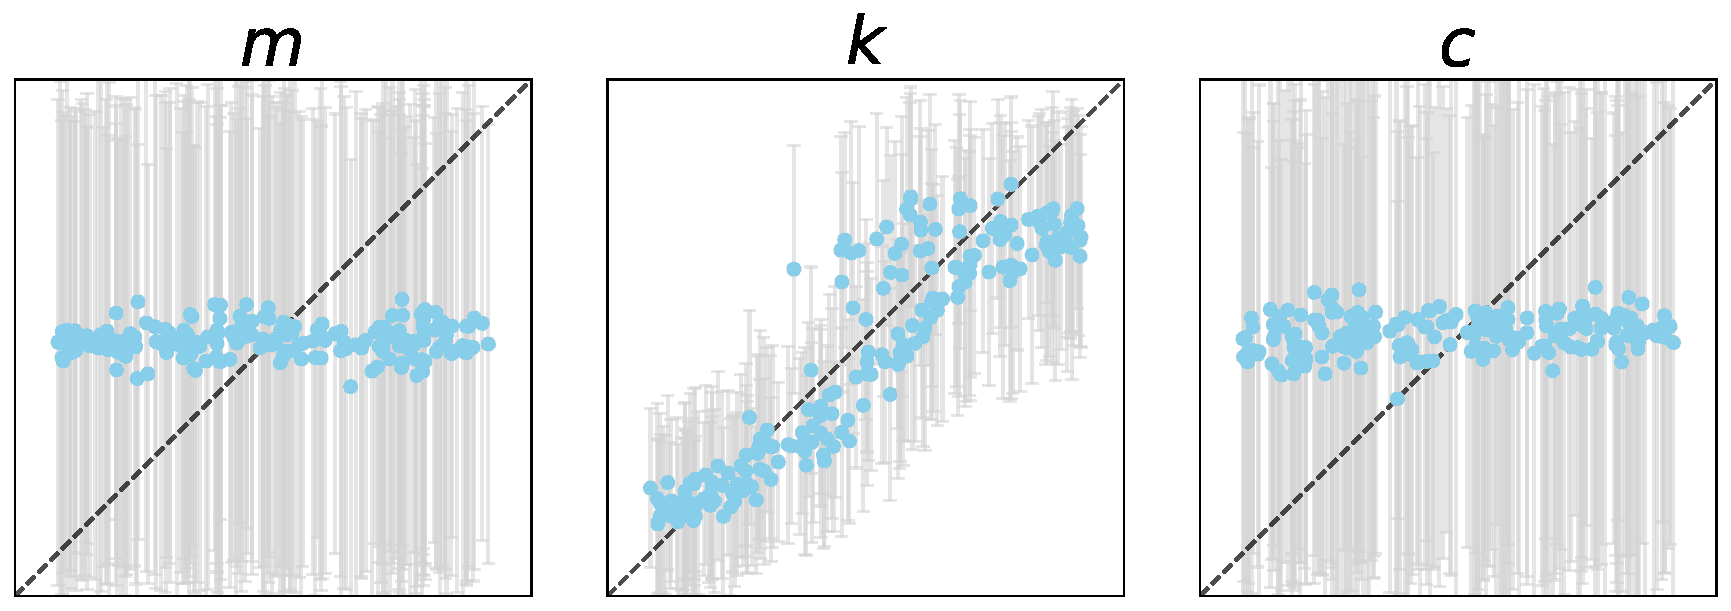
\includegraphics[width=\textwidth]{figures/RealNVP_mass_spring_damper_0.05_1.0_force_29.pdf}
        \caption{Epoch=29}
        \label{fig:sa_01}
    \end{subfigure}
    \hfill
    \begin{subfigure}[b]{0.48\textwidth}
        \centering
        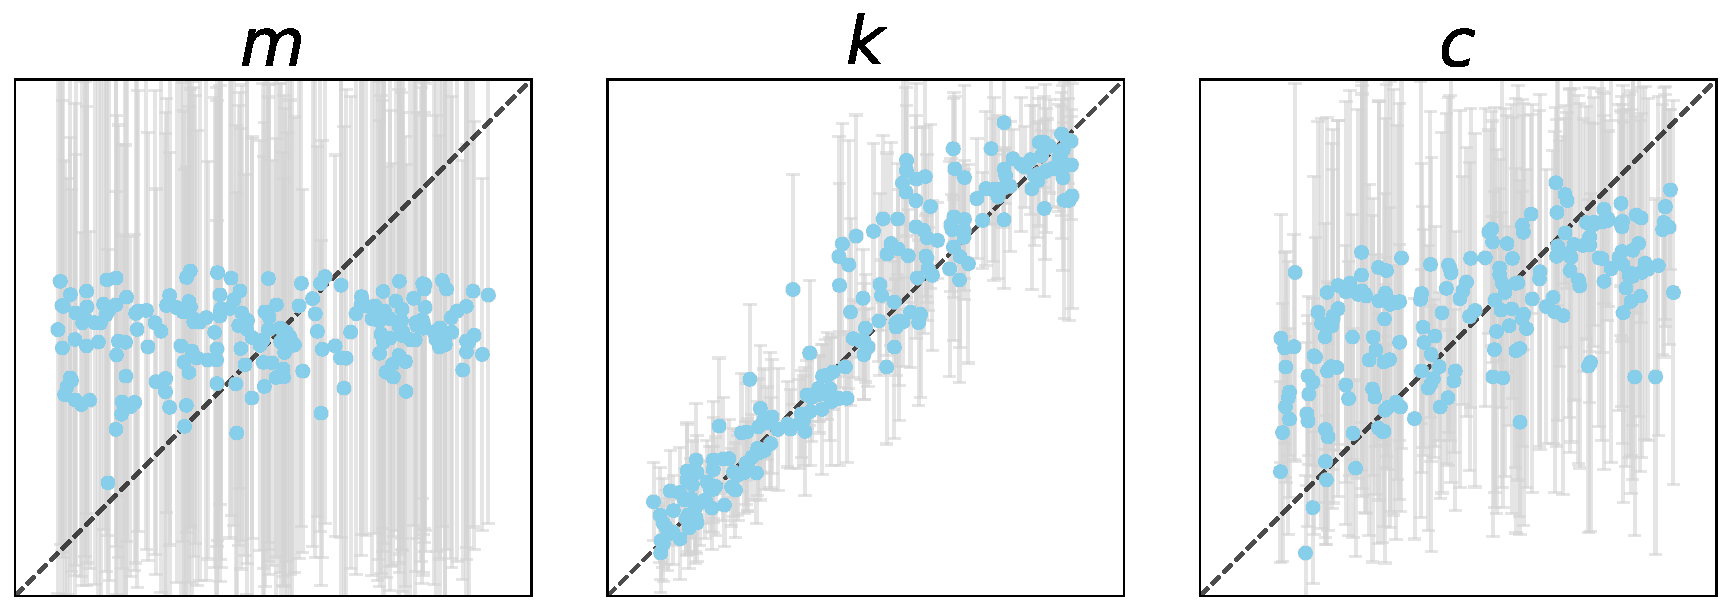
\includegraphics[width=\textwidth]{figures/RealNVP_mass_spring_damper_0.05_1.0_force_258.pdf}
        \caption{Epoch=258}
        \label{fig:sa_02}
    \end{subfigure}

    \begin{subfigure}[b]{0.48\textwidth}
        \centering
        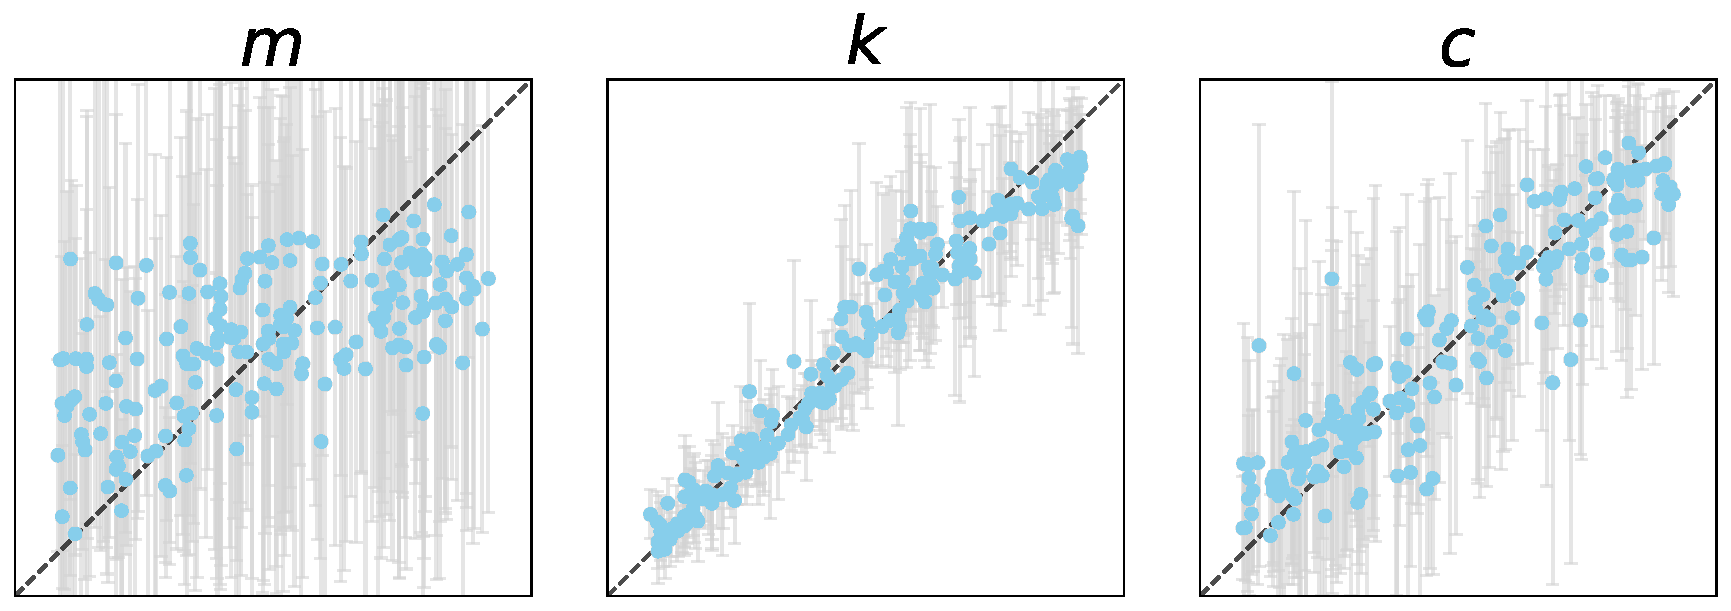
\includegraphics[width=\textwidth]{figures/RealNVP_mass_spring_damper_0.05_1.0_force_393.pdf}
        \caption{Epoch=393}
        \label{fig:sa_03}
    \end{subfigure}
    \hfill
    \begin{subfigure}[b]{0.48\textwidth}
        \centering
        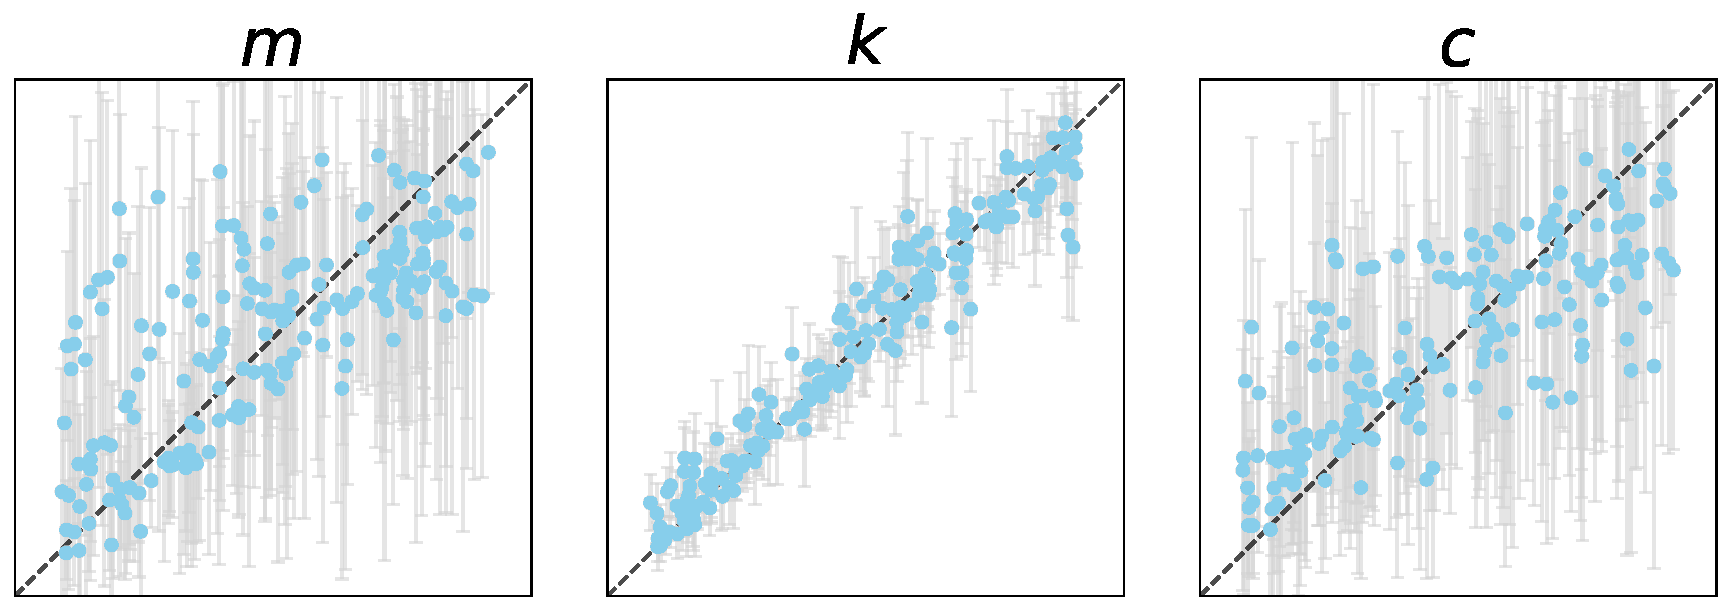
\includegraphics[width=\textwidth]{figures/RealNVP_mass_spring_damper_0.05_1.0_force_951.pdf}
        \caption{Epoch=951}
        \label{fig:sa_04}
    \end{subfigure}

    \caption[Convergence Speed \& Sensitivity Analysis]{Parameter identification results of \ac{RealNVP} at the early training stages. The figures show the estimation results of parameters $m,k,c$. The horizontal axis represents the ground truth, while the vertical shows the estimated values. The perfect convergence is demonstrated by the diagonal dashed line.}
    \label{fig:sa_speed}
\end{figure}

Figure~\ref{fig:sa_speed} illustrates the convergence behavior of the three parameters during the early stages of training. By the 29th epoch, the stiffness $k$ begins to converge toward the diagonal parity line, whereas the other two parameters remain unresolved, centered at the mean of their respective ranges. At the 258th epoch, $c$ begins to show a slight tendency toward convergence, while $k$ is further refined; however, $m$ shows no significant improvement. By the 393rd epoch, $m$ also begins to converge. Finally, at the 951st epoch, $m$ and $c$ reach a similar level of accuracy, while the estimate for $k$ continues to improve. This development reflects the sensitivity of parameters. It is worth noting that faster convergence of $c$ than $m$ results from the larger data range of $c$. The convergence speed of both parameters eventually synchronizes. 

\begin{figure}[htbp]
    \centering
    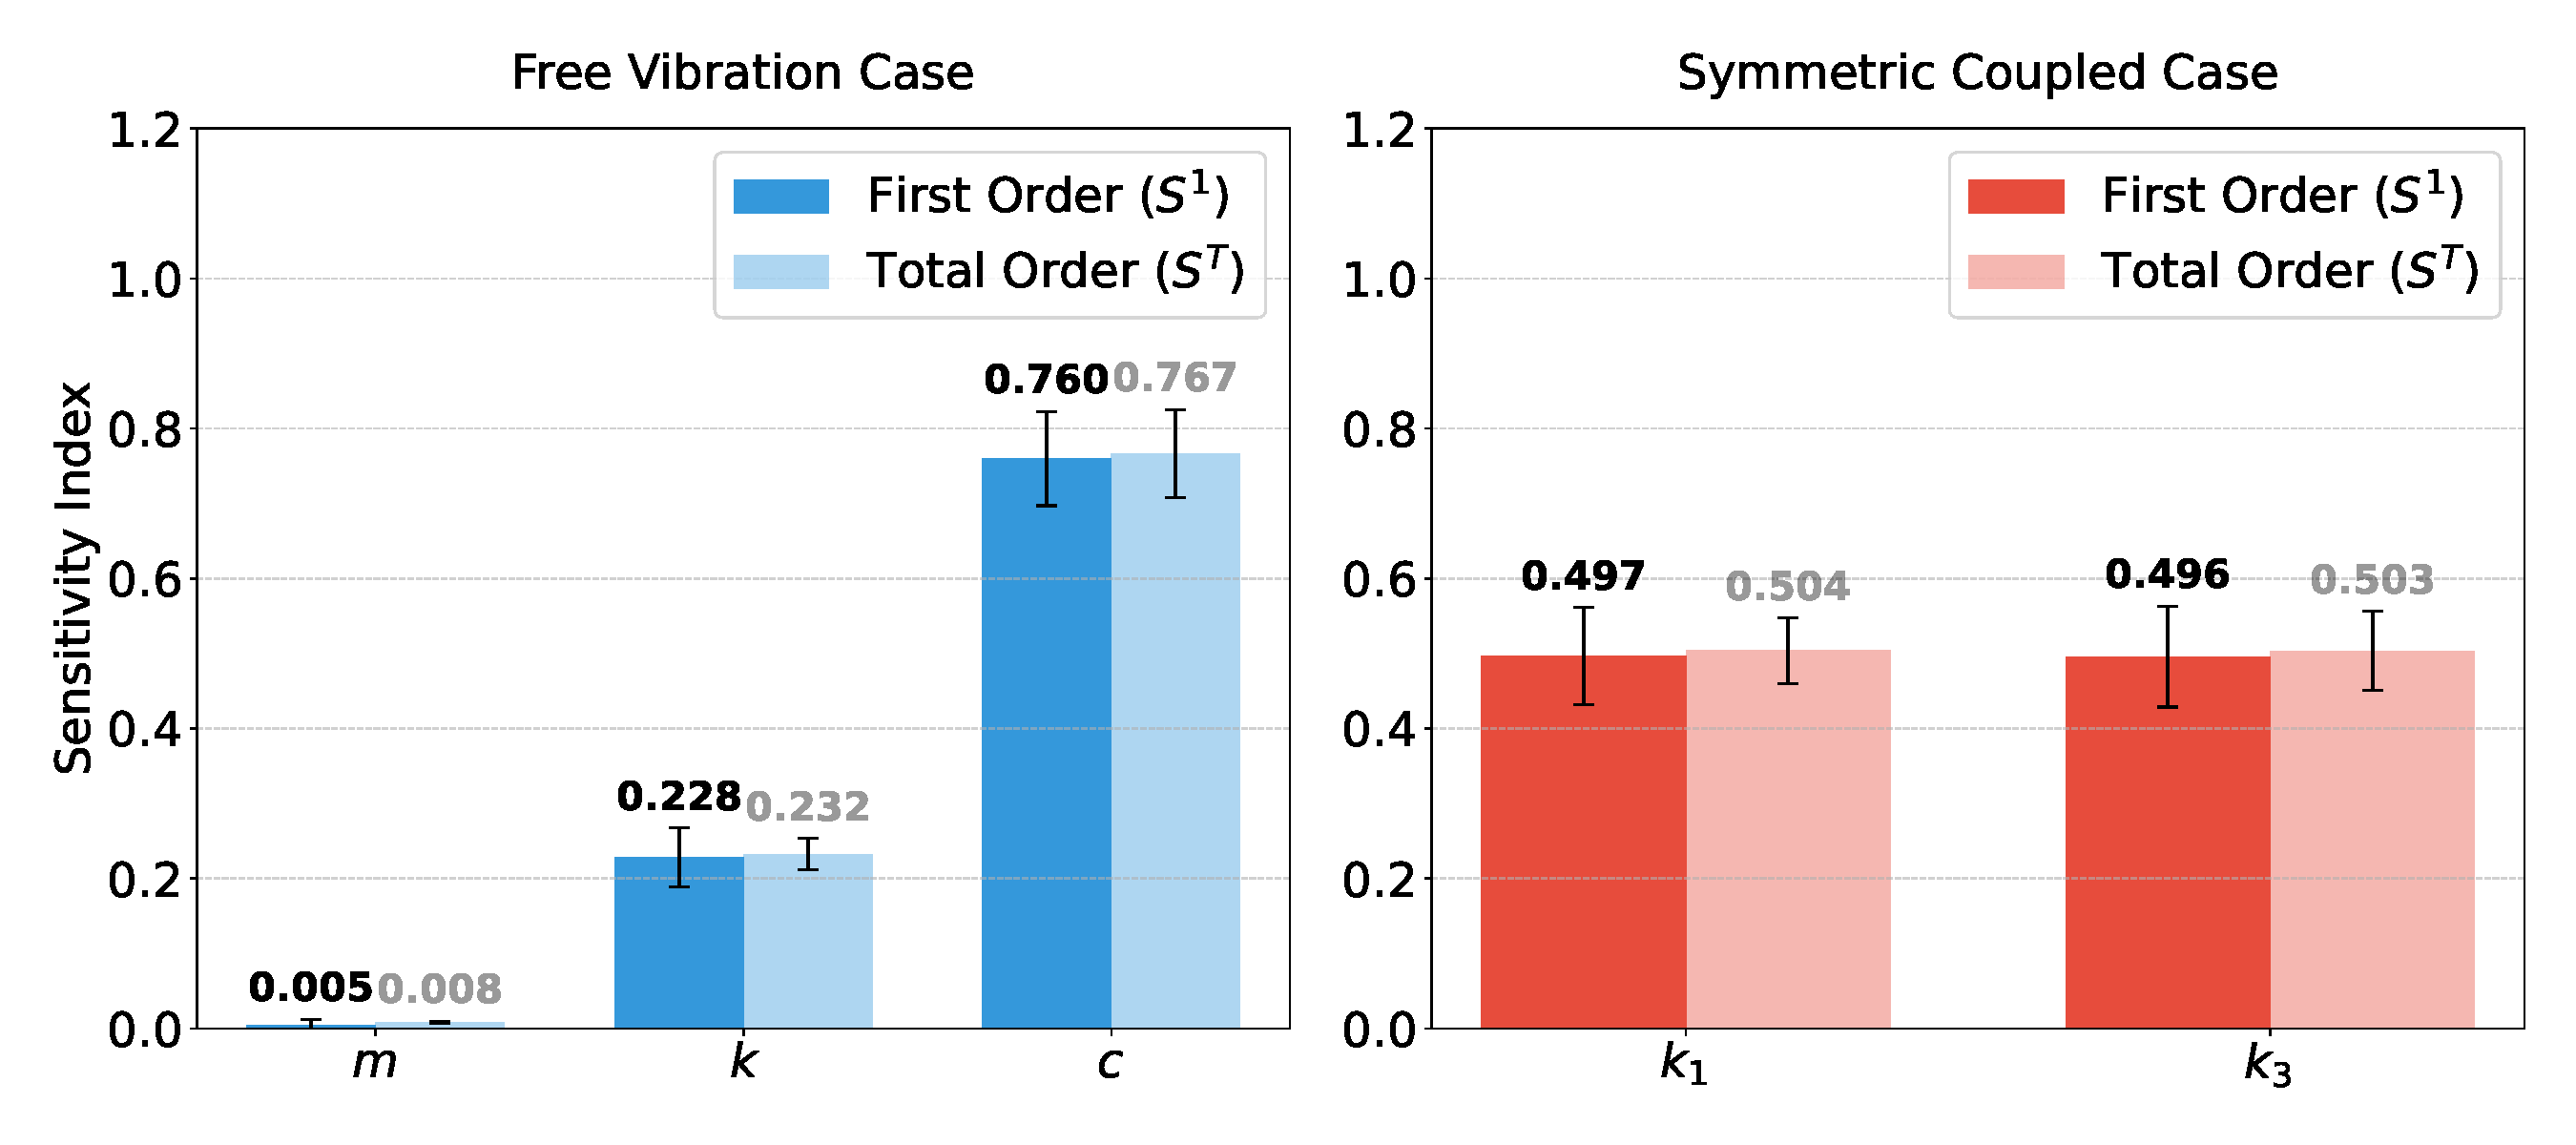
\includegraphics[width=0.9\textwidth]{figures/sensitivity_analysis_linear_coupled.pdf}
    \caption[Global Sensitivity Analysis of Free-Vibration and Symmetric Coupled Mass-Spring-Models]{Global \ac{SA} comparison in free-vibration and symmetric coupled mass-spring-damper systems. The bar charts display the first-order ($S^1$) and total-order ($S^T$) Sobol’ indices, with error bars representing the 95\,\% confidence interval. (Left) In the free-vibration case, the parameters $m,k,c$ have highly different sensitivities. (Right) In the symmetric coupled two-mass system, $k_1$ and $k_3$ exhibit nearly identical sensitivity.}
    \label{fig:sa_l_c}
\end{figure}

Figure~\ref{fig:sa_l_c} compares the sensitivity analysis of the free and coupled mass-spring-models. In the free-vibration case, the external force is removed. The behavior of the mass-spring-model is heavily influenced by how fast the energy loses, which is caused by the damping $c$. The global \ac{SA} of the free-vibration system reveals a clear hierarchy of parameter identifiability. The damping coefficient  $c$ dominates the output variance ($S^T_c=0.767$), followed by the stiffness $k$ ($S^T_k=0.232$), and the mass $m$ exhibits negligible sensitivity ($S^T_m=0.008$). Furthermore, the near-equality of $S^1$ and $S^T$ across all parameters indicates a lack of higher-order interactions. This suggests $m$ is weakly identifiable, whereas the other two parameters can be identified independently. 

The global \ac{SA} of the symmetric coupled two-mass system reveals a perfect parity between the boundary stiffness parameters. Both $k_1$ and $k_3$ exhibit nearly identical first-order ($S^1\approx 0.496$) and total-order ($S^T\approx 0.503$) indices. The near-unity sum of their first-order indices ($S_{k_1}+S_{k_3}\approx 1$) suggests that these two parameters account for almost the entire variance of the system's dynamic response, with negligible higher-order interactions ($S^T-S^1<0.01$). From an identifiability perspective, this symmetry presents a unique challenge for Bayesian inference. While the high sensitivity ensures that the parameters will converge quickly away from the prior mean, the identical nature of their influence results in a bimodal posterior distribution. This confirms the indistinguishability and multimodality: the amortized inference model can identify the required stiffness levels but cannot uniquely assign them to $k_1$ or $k_3$ without additional asymmetric constraints or localized observations.

\subsubsection{Mutual Information}
Global \ac{SA} does not always provide a reliable measure of parameter identifiability, particularly when observations are corrupted by additive noise. Consider a model $f(\boldsymbol{X})$ whose observations contain additive Gaussian noise $\epsilon\sim N(0,\sigma_n^2)$, such that $Y=f(\boldsymbol{X})+\epsilon$. Assuming the noise is independent of the parameters, the total observed variance becomes $Var(Y)=Var(f(\boldsymbol{X}))+\sigma_n^2$. Under this condition, the first-order and total-order Sobol' indices behave differently:
\begin{align}
    S^1_i &= \frac{V_i}{Var(Y)+\sigma^2_n} < \frac{V_i}{Var(Y)};\\ 
    S^T_i &= \frac{Var_{\boldsymbol{X}_{\backslash i}}[E_{X_i}(Y|\boldsymbol{X}_{\backslash i})]+\sigma_n^2}{Var(Y)+\sigma_n^2}>\frac{Var_{\boldsymbol{X}_{\backslash i}}[E_{X_i}(Y|\boldsymbol{X}_{\backslash i})]}{Var(Y)}.
\end{align}
As the noise ratio increases, the first-order Sobol' index decreases because the denominator grows while the numerator remains constant. In contrast, the total-order Sobol' index increases by adding the variance of noise in both numerator and denominator. This behavior is highly counter-intuitive: a higher total Sobol' index usually suggests that a parameter is more influential, yet in this case, the increase is driven entirely by noise, which actually makes the parameter more difficult to identify. Consequently, variance-based metrics can fail to distinguish between true parameter sensitivity and the presence of measurement uncertainty. To address these limitations, \ac{MI} \citep{Bhola2023-ik} offers a robust alternative for evaluating the practical identifiability of parameters. Unlike global \ac{SA}, which only considers the second moment (variance), \ac{MI} is an information-theoretic measure that quantifies the total information gain from the prior to the posterior distribution given the data:
\begin{equation}
MI(X_i, y) = H(p(X_i)) - H(p(X_i|y)),
\end{equation}

\begin{figure}[htbp]
    \centering
    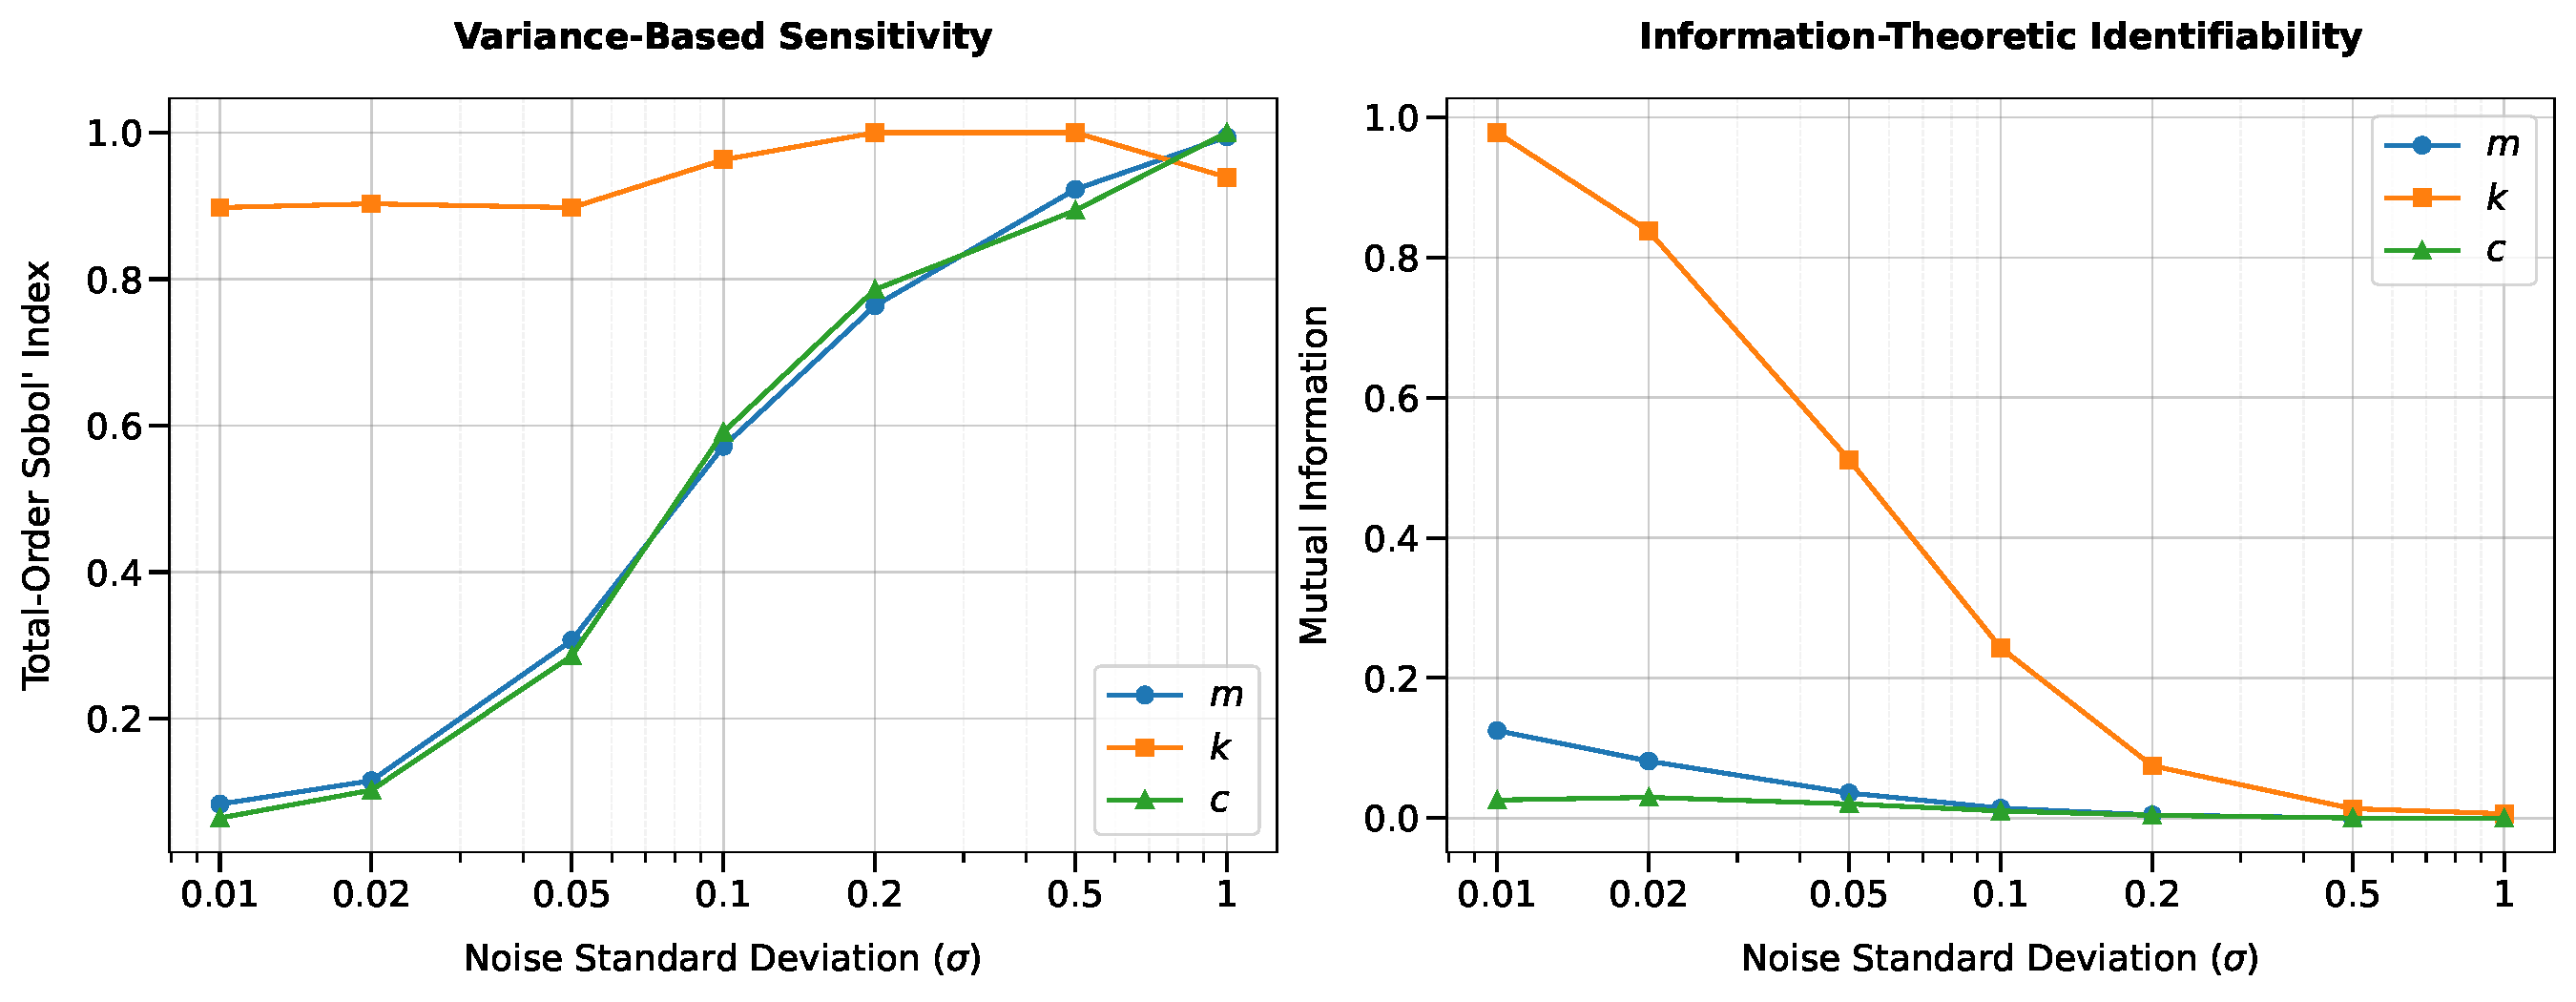
\includegraphics[width=\textwidth]{figures/sensitivity_identifiability.pdf}
    \caption[Comparison of Sensitivity and Identifiability Under Noisy Observations]{Comparison of parameter sensitivity and identifiability under varying noise levels. The left panel displays the total-order Sobol' index, while the right panel shows the Mutual Information (MI) for the parameters $m,k,c$ of a forced mass-spring-damper model. Both metrics were estimated using \num{1024} samples generated from a low-discrepancy sequence. The horizontal axis represents the noise ratio (scaling a standard normal distribution) on a logarithmic scale.}
    \label{fig:mi_noise}
\end{figure}

A comparison between the total-order Sobol' index and \ac{MI} across varying noise levels is shown in Figure \ref{fig:mi_noise}. While $S^T$ suggests a rising sensitivity as $\sigma$ increases, which results from the noise contributing to the total variance, the $MI$ captures the actual degradation of the signal-to-noise ratio. The divergence between these metrics demonstrates that sensitivity can be a misleading proxy for identifiability in noisy environments. Beyond a threshold of $\sigma=0.02$, the sharp drop in $MI$ indicates that the parameters cannot be identified as perfectly as the clean observations. Beyond a threshold of $\sigma=0.2$, all parameters are poorly identifiable, meaning the observations no longer provide sufficient information to constrain the prior.

\subsection{When Does the Framework Fail?}
From the previous sections, we have known the framework frequently struggles with posterior identifiability; specifically, when the system exhibits multimodality, generative models may fail to resolve disjoint parameter regimes. Apart from identifiability, the efficacy of amortized Bayesian inference via deep generative models is intrinsically tied to the fidelity of the latent representations extracted by the condition network. This framework encounters significant bottlenecks under three primary conditions. First, in the presence of high-dimensional, noisy, or highly stochastic time-series data, the condition network often fails to distill sufficient summary statistics, leading to information loss. Second, the framework is susceptible to model misspecification. When a discrepancy exists between the training simulator and real-world dynamics (the sim-to-real gap), the amortized posterior yields biased and poorly calibrated estimates. Third, the framework fails to generalize to parameter ranges outside its training boundaries, even if the underlying physics remain the same. 

We evaluate the robustness of \acp{NF} (including \ac{FM}, \ac{RealNVP}, and \ac{NSF}) by subjecting the framework to the following stress-test scenarios:
\begin{itemize}
\item Information Extraction Bottlenecks: Increasing observational noise to assess the limits of the condition network's feature extraction.
\item Structural Misspecification: Evaluating models trained on linear dynamics against data generated from non-linear physical systems.
\item \ac{OOD} Generalization: Testing the framework on parameter ranges that lie outside the support of the training prior.
\end{itemize}

\begin{figure}[htbp]
    \centering
    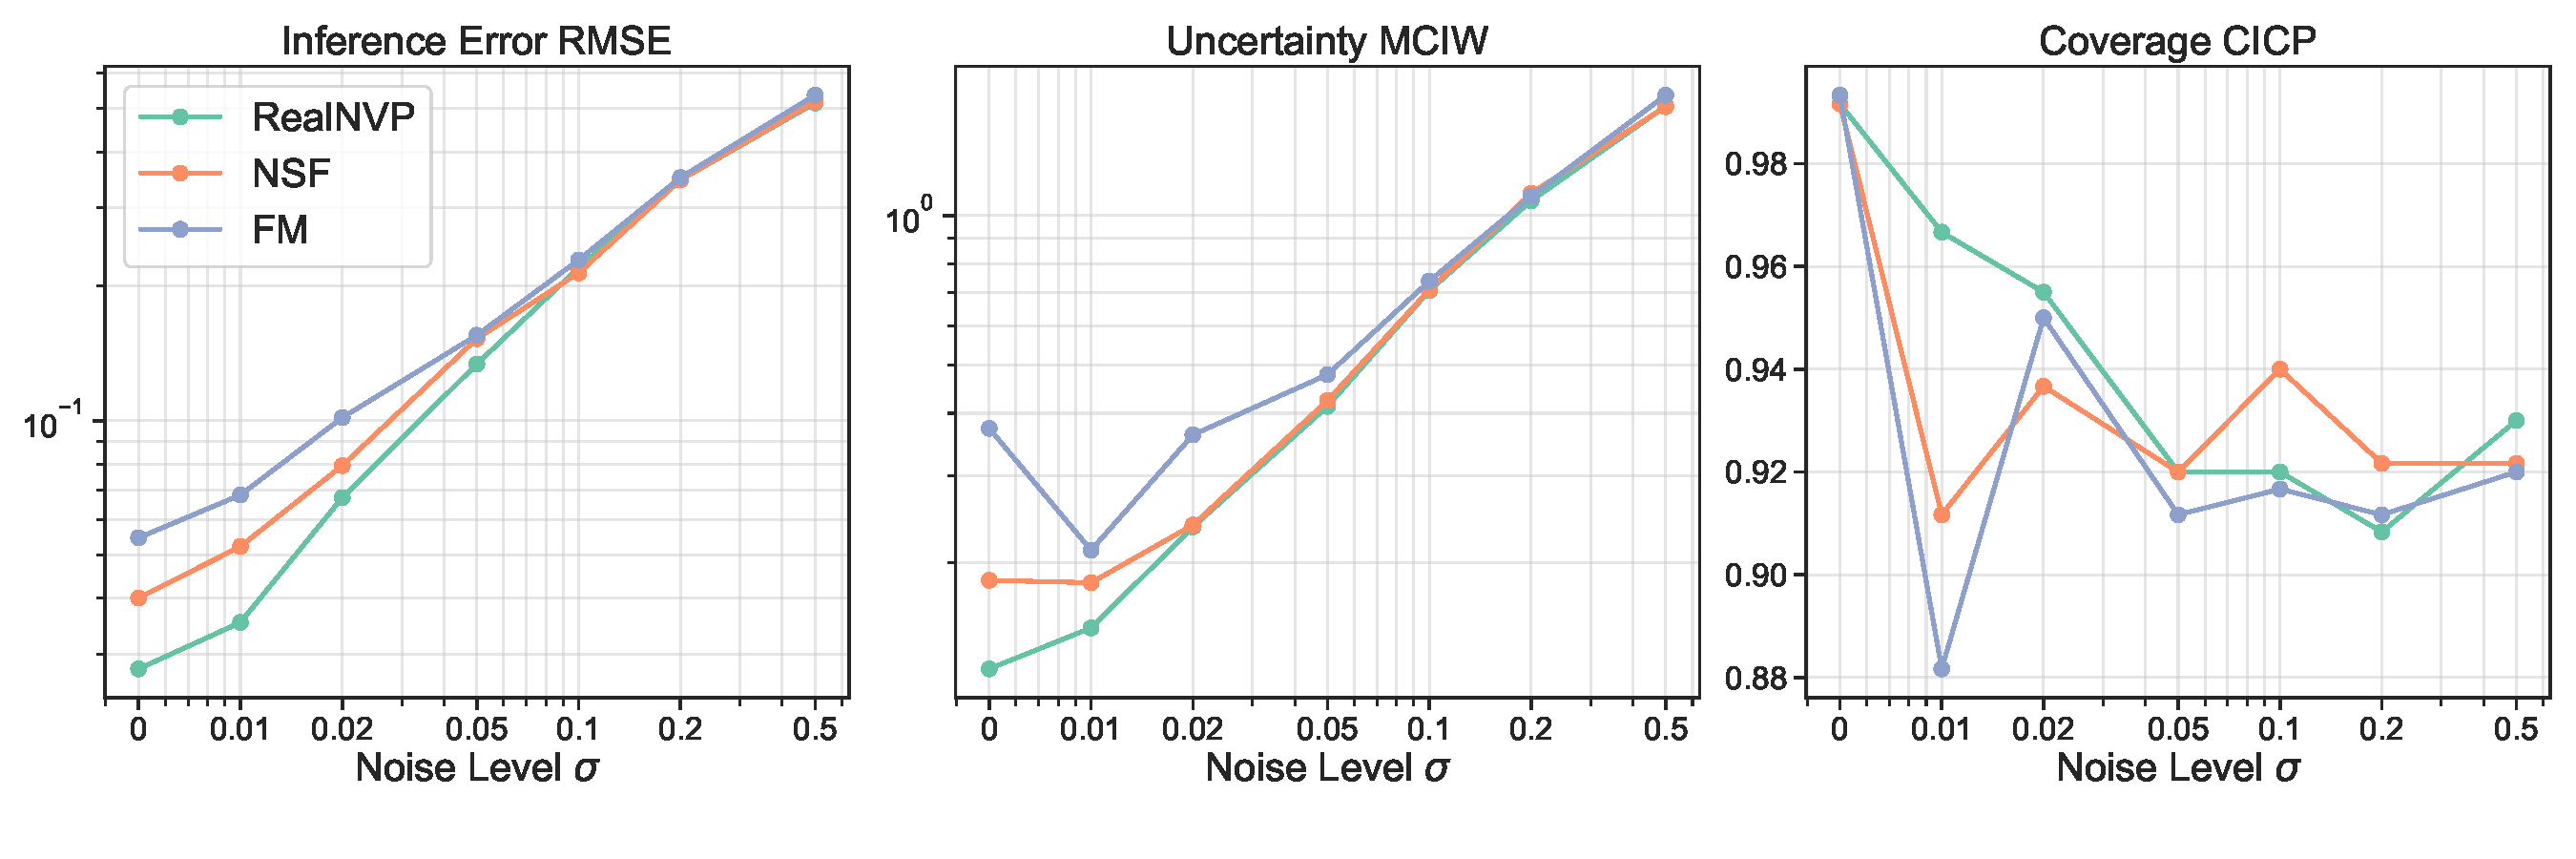
\includegraphics[width=\textwidth]{figures/stress_test_noise.pdf}
    \caption[Stress Test of Normalizing Flows under Noise]{Stress test of Normalizing Flow architectures under increasing additive Gaussian noise. The panels illustrate the evolution of predictive accuracy (RMSE), uncertainty quantification (MCIW), and posterior calibration (CICP) for \ac{RealNVP}, \ac{NSF}, and \ac{FM} as the noise intensity $\sigma$ changes. Logarithmic scaling is applied to both the noise level and the corresponding RMSE and MCIW metrics to highlight performance degradation across several orders of magnitude.}
    \label{fig:st_noise}
\end{figure}

Figure~\ref{fig:st_noise} illustrates the performance of the three \ac{NF} architectures under varying levels of additive Gaussian noise $\sigma$. At the low-noise level ($\sigma=0.01$), all models exhibit a sharp decline in coverage probability, particularly the \ac{FM} and \ac{NSF} variants. This indicates a calibration failure where the condition network fails to fully distinguish observational stochasticity from parameter variance, leading to overly confident (narrow) posteriors. As noise intensity increases beyond $\sigma=0.05$, the models show a monotonic degradation in accuracy (RMSE) accompanied by a proportional expansion of uncertainty (MCIW). In the high-noise range ($\sigma\ge0.05$), the models converge in behavior, successfully broadening their posterior estimates to maintain a stable, albeit lower, coverage floor of approximately 0.92.

\begin{figure}[htbp]
    \centering

    \begin{subfigure}[b]{0.49\textwidth}
        \centering
        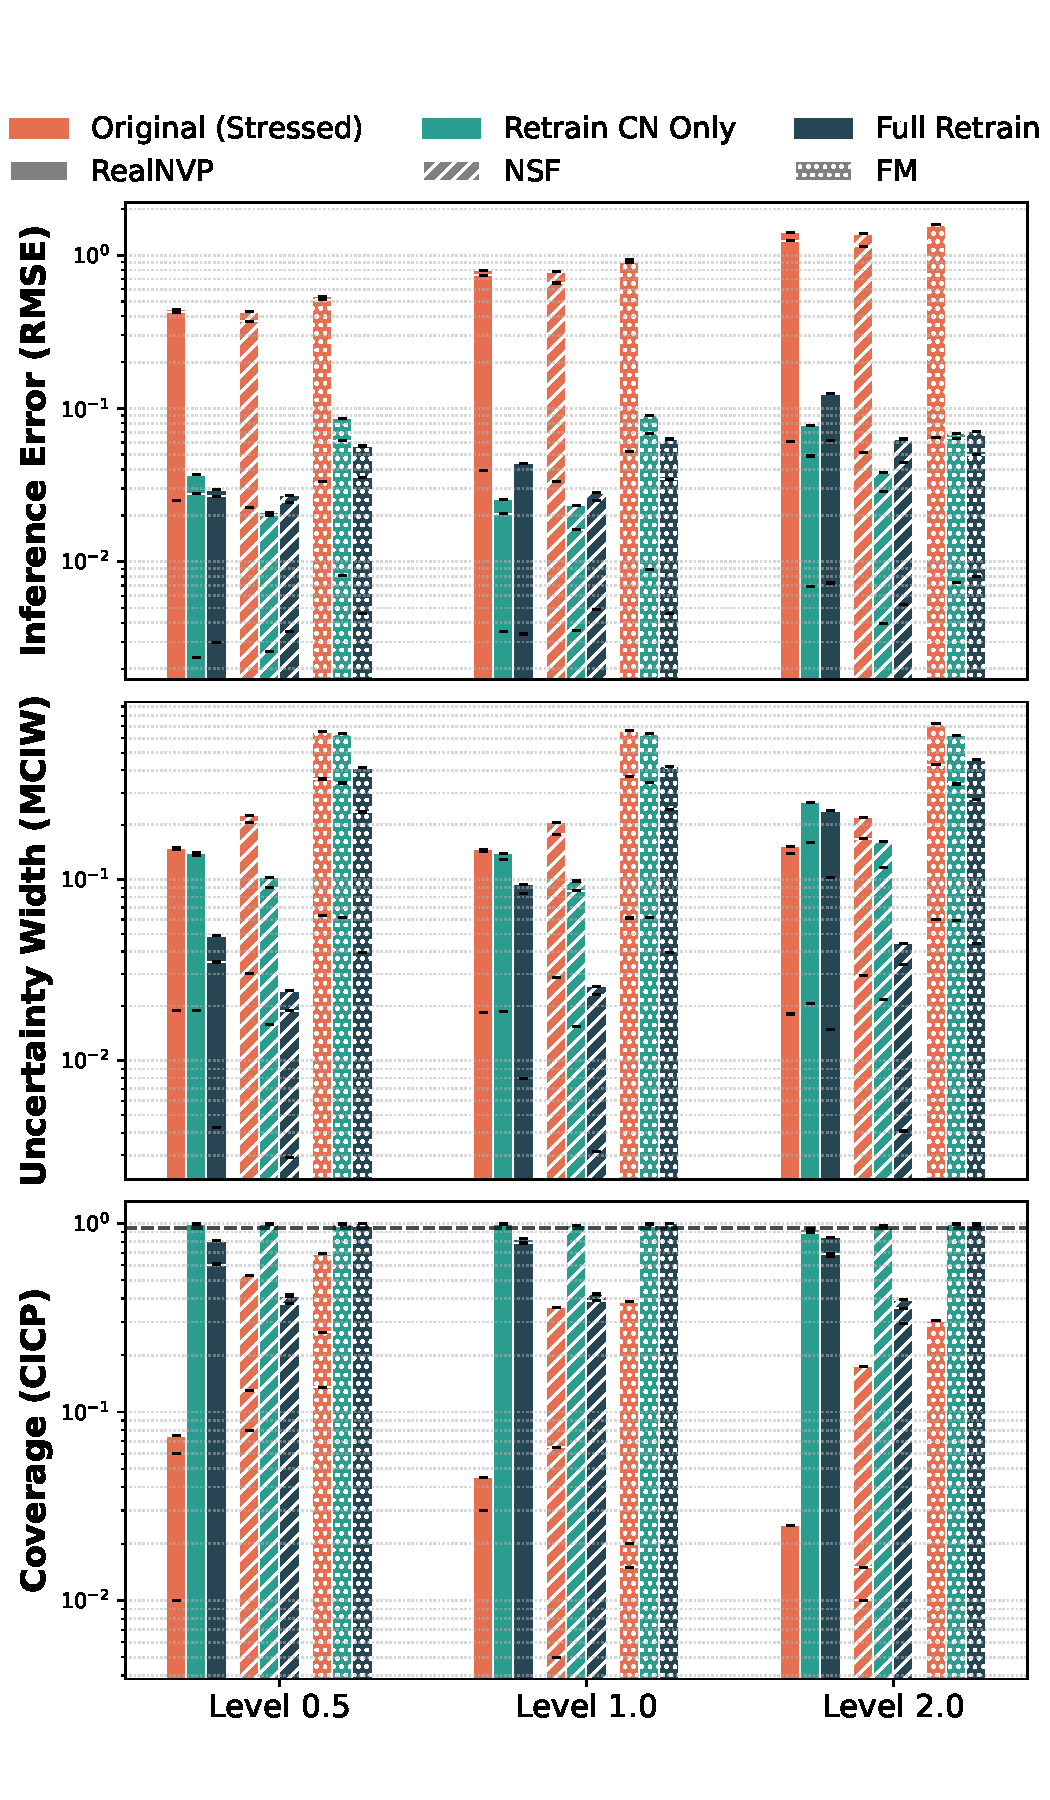
\includegraphics[width=\textwidth]{figures/misspecification_metrics.pdf}
        \caption{Misspecification}
        \label{fig:miss_metrics}
    \end{subfigure}
    \hfill
    \begin{subfigure}[b]{0.50\textwidth}
        \centering
        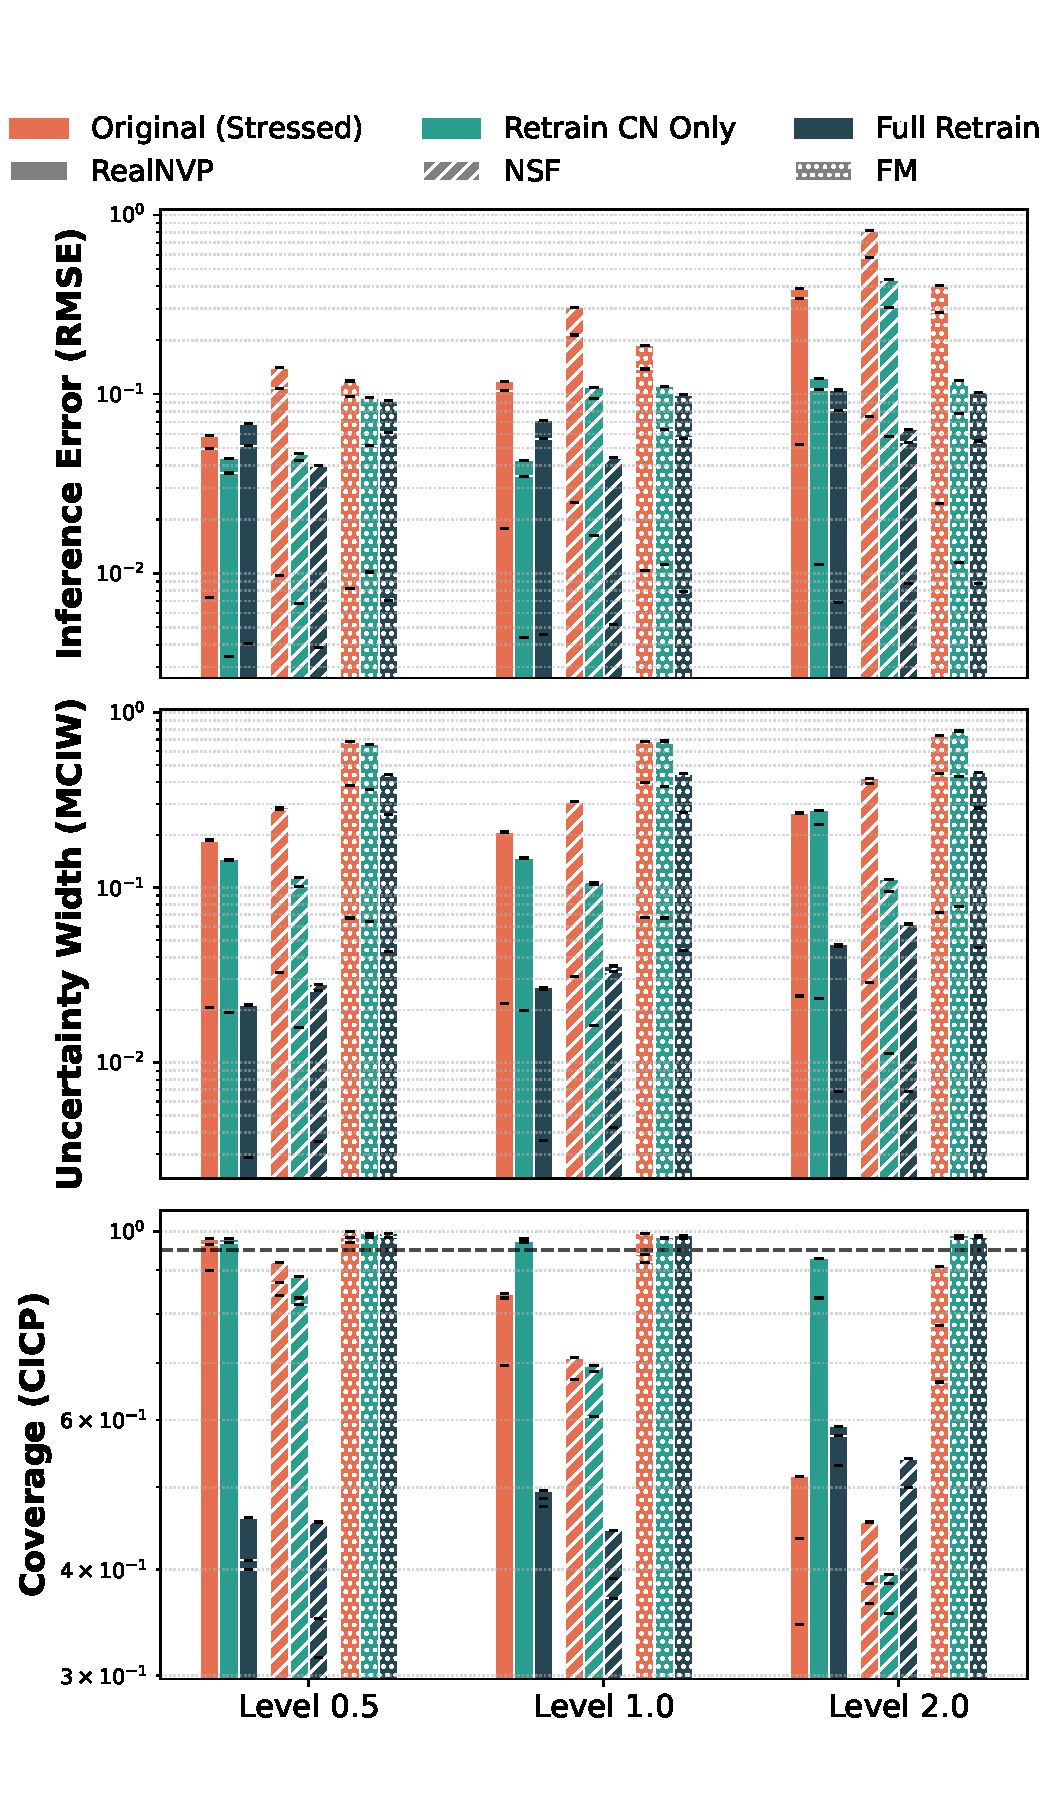
\includegraphics[width=\textwidth]{figures/ood_metrics.pdf}
        \caption{OOD}
        \label{fig:ood_metrics}
    \end{subfigure}

    \caption[Evaluation of Stress Test under Misspecification and OOD]{Evaluation of model performance under structural misspecification and \ac{OOD} stress tests. Rows from top to bottom display inference accuracy (RMSE), uncertainty estimation (MCIW), and coverage probability (CICP). The dashed line in CICP subfigure shows 0.95 coverage probability. Metric values are averaged across \num{200} test scenarios and three mechanical parameters ($m,k,c$). The grouped bar plots illustrate performance at varying stress levels $0.5, 1, 2$. For structural misspecification, the level corresponds to the magnitude of the nonlinear factor $\beta$ introduced into the system dynamics: $\dot v = (F_t - kx + \beta x^3 - cv+\beta v |v|)/m$. For \ac{OOD} testing, the level denotes the shift $\Delta$ of the test data range relative to the original training set, where $\Delta=(+0.1\alpha, +\alpha, +0.5\alpha)$. At each level, colors indicate the training state: the original baseline under stress, and the improved results after retraining either the condition network or the entire network. Bar patterns represent the normalizing flow architecture (RealNVP, NSF, and FM).}
    \label{fig:metrics}
\end{figure}

\begin{figure}[htp!]
    \begin{minipage}{0.65\textwidth}
        \centering
        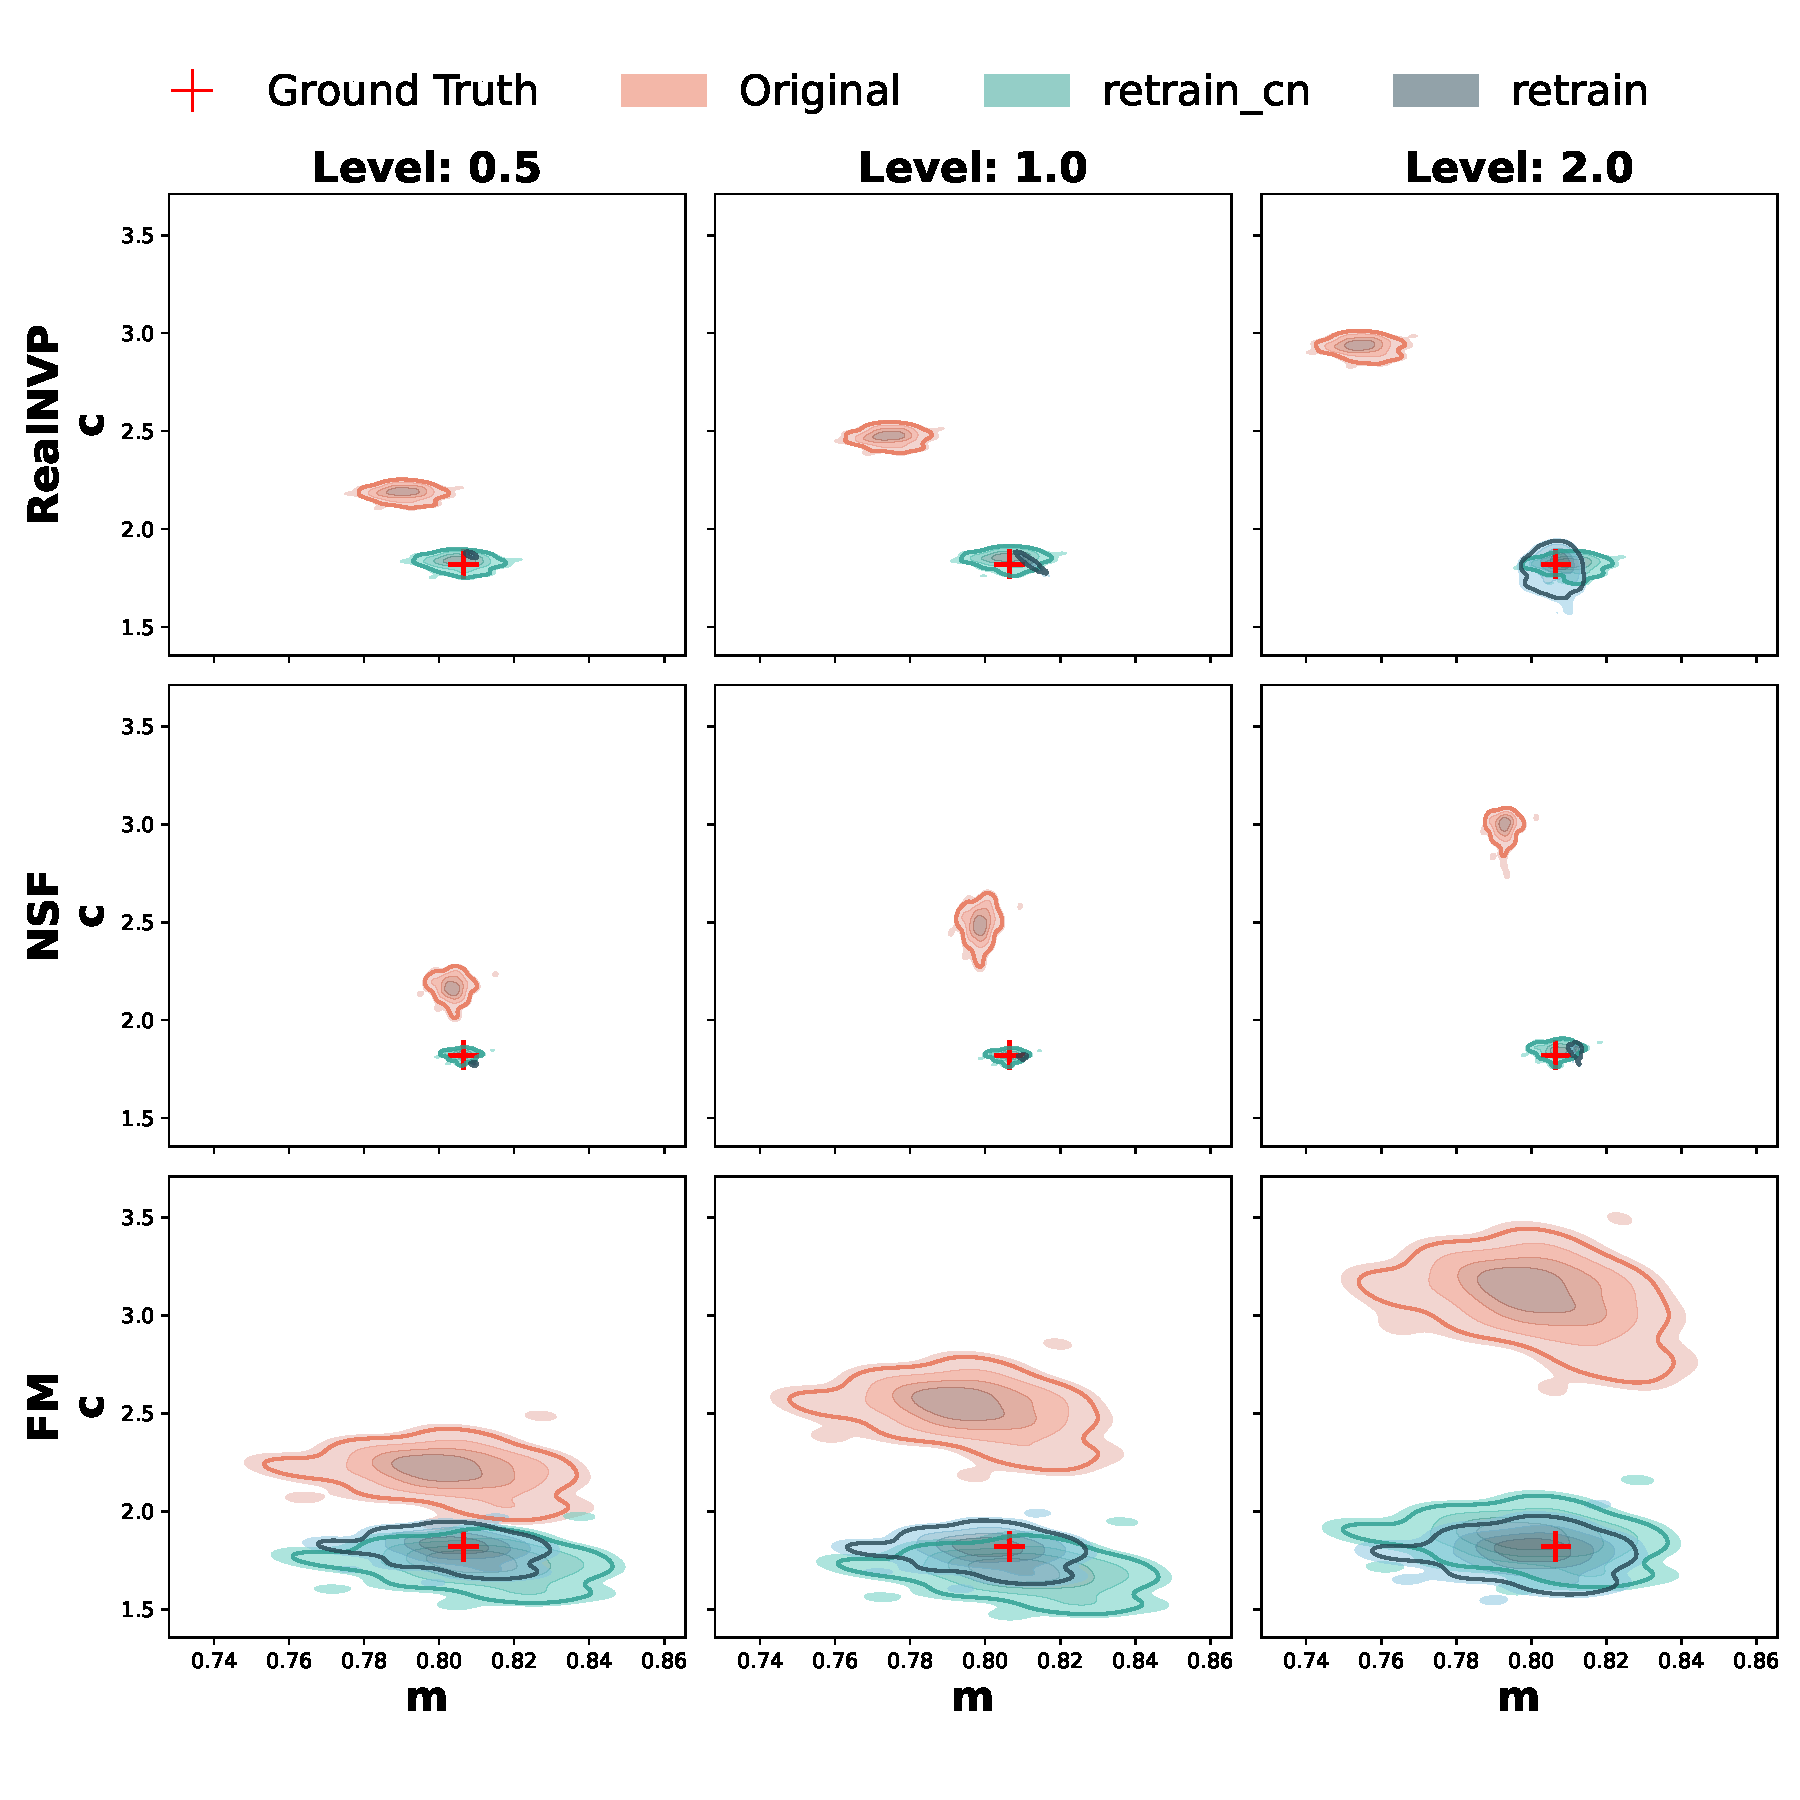
\includegraphics[width=\linewidth]{figures/misspecification_distribution.pdf}
      \end{minipage}
      \hfill
    \begin{minipage}{0.32\textwidth}
    \caption[Micro View of Distribution under Misspecification]{Micro View of posterior distributions under misspecification for a single test scenario. The 3×3 grid illustrates the joint posterior distributions of parameters $m$ and $c$ across three architectures (RealNVP, NSF, and FM) and three misspecification levels ($\beta=0.5, 1, 2$). Colors represent the model state: the baseline under stress (Original), the improved result after retraining the condition network (retrain-cn), and the result after full-network retraining (retrain). The ground truth is marked by a red cross (+). }
    \label{fig:miss_distribution}
    \end{minipage}
\end{figure}

\begin{figure}[htp!]
    \begin{minipage}{0.65\textwidth}
        \centering
        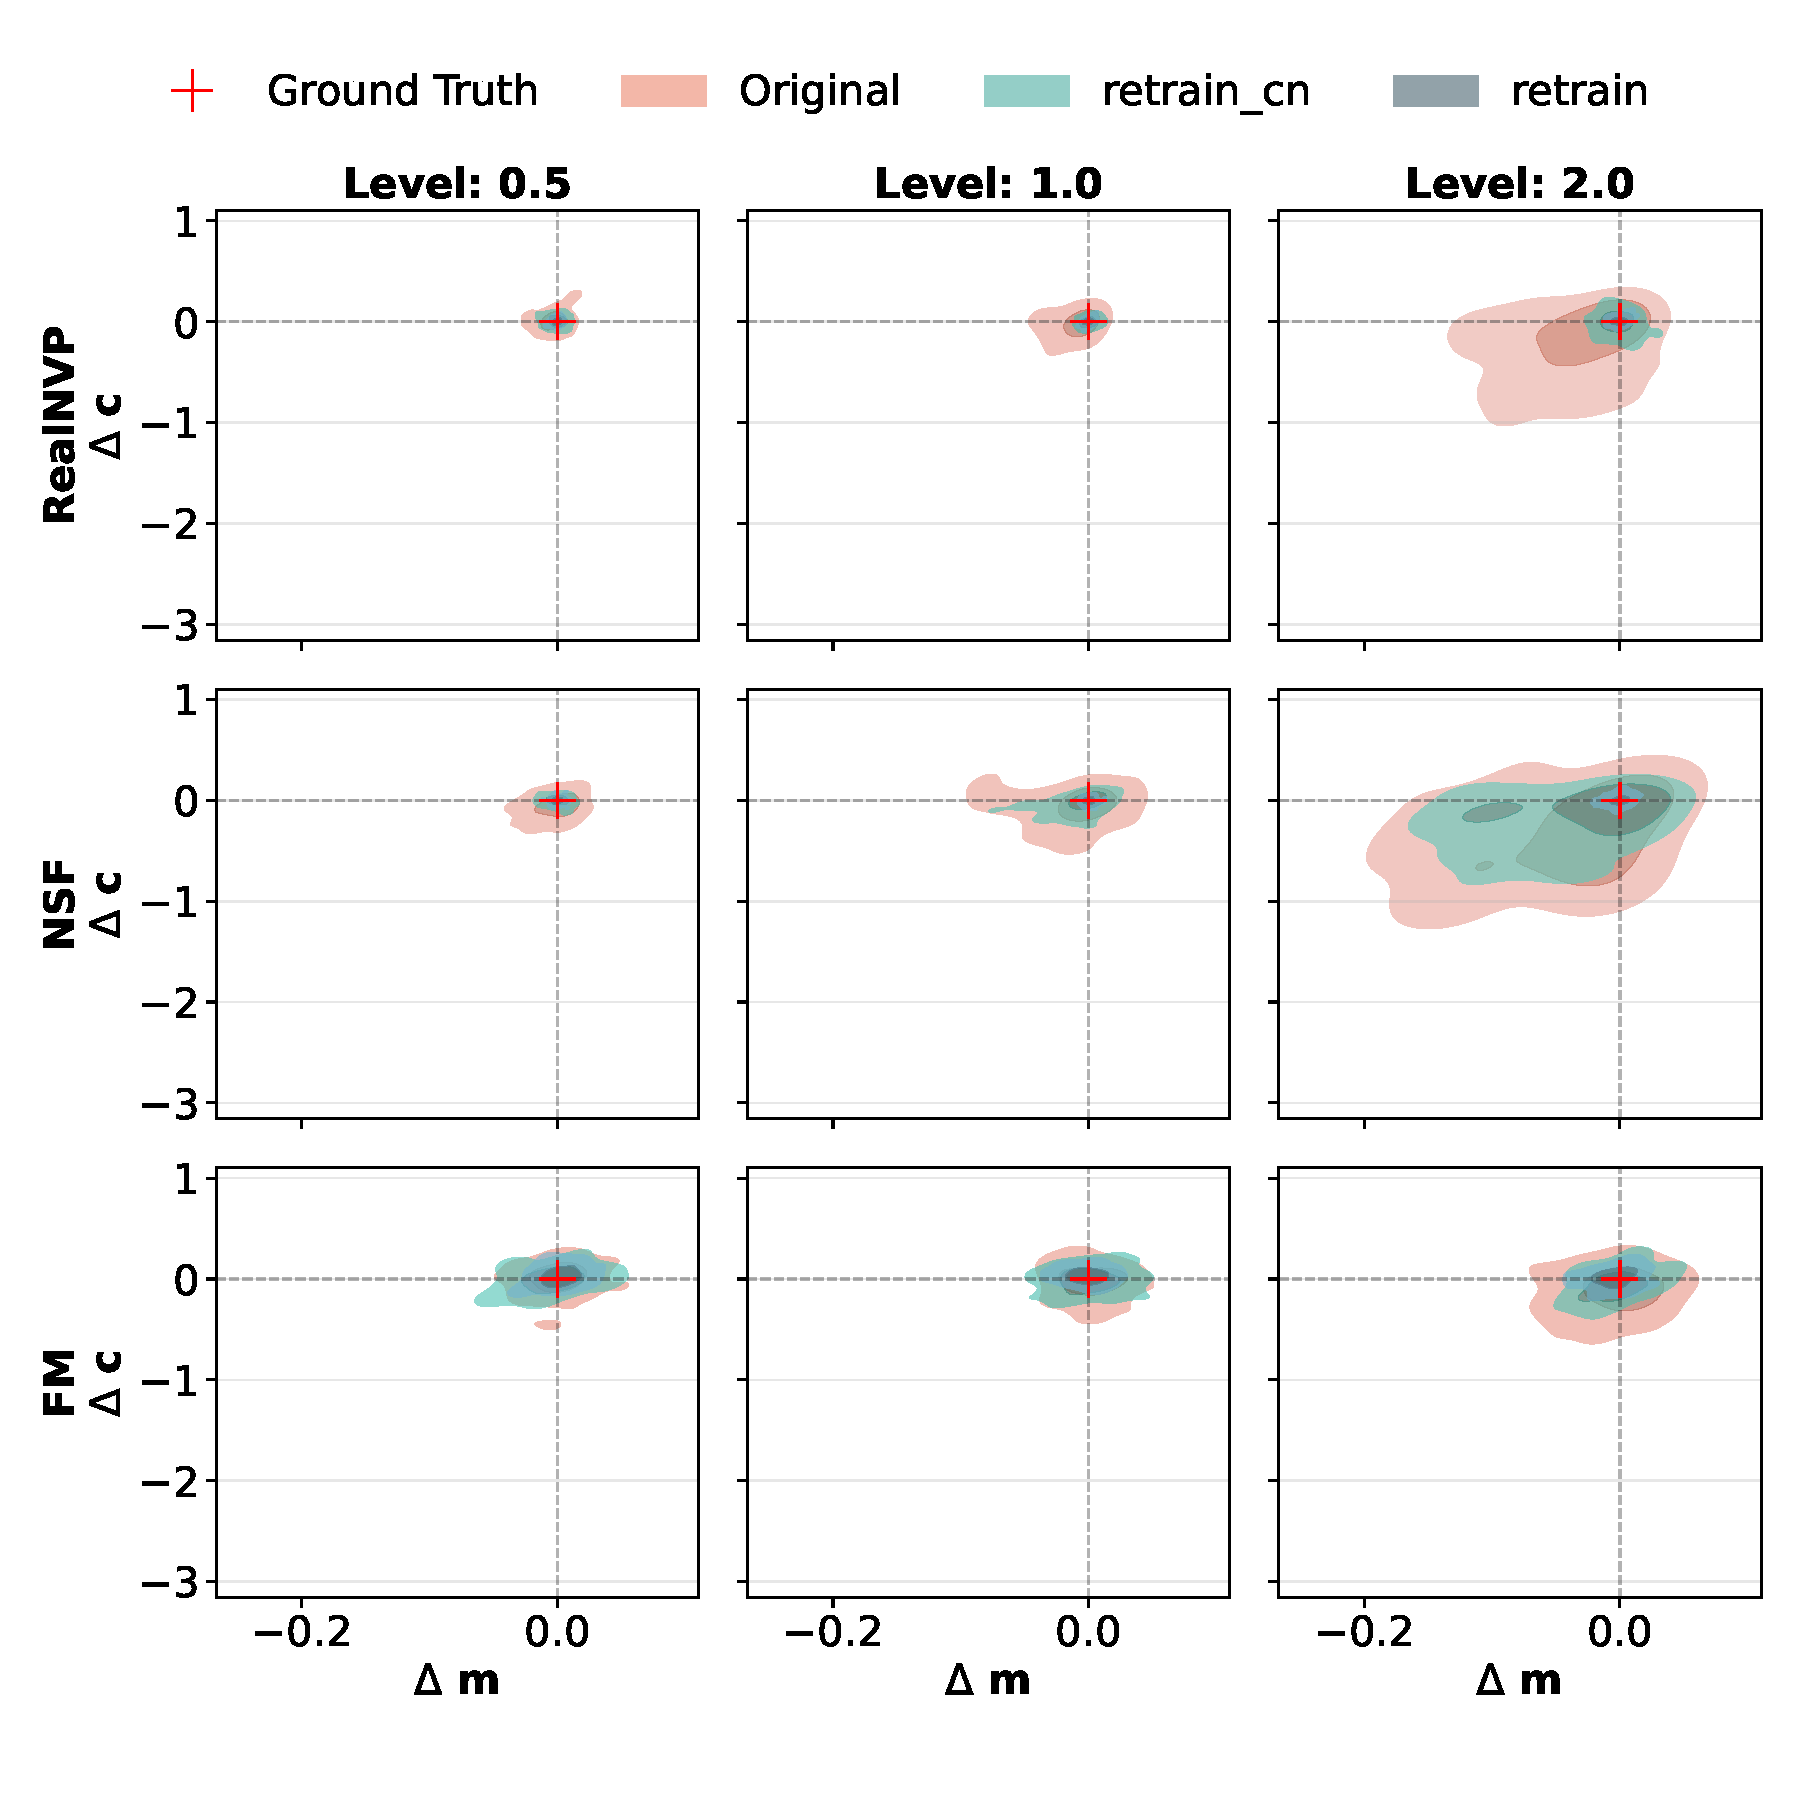
\includegraphics[width=\linewidth]{figures/ood_residual.pdf}
      \end{minipage}
      \hfill
    \begin{minipage}{0.32\textwidth}
    \caption[Global Residual Analysis under OOD]{Global residual analysis under \ac{OOD} for 200 test scenarios. The 3×3 grid illustrates a global residual analysis of the joint distributions for mass $\Delta m=\hat{m}-m$ and damping $\Delta c=\hat{c}-c$ across three architectures (RealNVP, NSF, and FM) and three \ac{OOD} levels ($\alpha=0.5, 1, 2$). Colors represent the model state: the baseline under stress (Original), the improved result after retraining the condition network (retrain-cn), and the result after full-network retraining (retrain). The perfect match (zero error) is marked by a red cross (+).}
    \label{fig:ood_distribution}
    \end{minipage}
\end{figure}

In such cases, the condition network encounters a representational bottleneck; it fails to extract sufficient summary statistics, preventing the observational variance from being accurately mapped to the parameter sensitivity. To mitigate this, an \ac{MCMC} algorithm can be employed to correct the estimates, using the amortized posterior as an informative proposal distribution. Alternatively, a more computationally efficient approach involves \ac{SNF}, which integrates the simulator directly into the latent transformation as a log-posterior diagnostic, as detailed in Section \ref{sec:snf}.

The structural misspecification and \ac{OOD} generalization problems can be solved by active learning, i.e., retraining the architectures with new data. Figure~\ref{fig:metrics} shows the improvement through model adaptation of misspecification and \ac{OOD} generalization, respectively. In both cases, comparing different retraining methods (different colors), updating only the condition network effectively centers the distribution, significantly reducing RMSE and bringing CICP back toward the 0.95 target. While retraining the whole networks produces the most improvement in terms of minimizing error and tightening confidence intervals, it carries the highest risk of overfitting the posterior. Comparing different flow architectures (different patterns), RealNVP and NSF achieve the lowest RMSE and narrowest MCIW after retraining. However, they are highly sensitive to the misspecification or \ac{OOD} stress. In contrast, FM shows higher inference error and wider uncertainty than others but maintains higher coverage probability. It is less prone to overfitting and resilient against the stress.

Figure~\ref{fig:miss_distribution} is a micro view of the joint distributions between $m$ and $c$ in a test scenario. As the stress level increases, a clear divergence from the ground truth is observed in the baseline models. While FM exhibits a larger posterior variance compared to the other architectures, it demonstrates superior robustness. Retraining the condition network successfully shifts the posteriors back toward the ground truth. However, full-network retraining for RealNVP and NSF leads to overconfidence; while point accuracy increases, the distributions shrink excessively, causing a drop in coverage. In contrast, FM retraining further constrains the distribution without inducing this overfitting effect, maintaining better calibration than the condition-network adaptation.

Figure~\ref{fig:ood_distribution} represents a global residual analysis under OOD. By centering the ground truth of each scenario at $(0,0)$, the subplots reveal the systematic bias and uncertainty induced by increasing \ac{OOD} shifts. As the shift increases from 0.5 to 2.0, the Original baseline distributions exhibit both a significant expansion in variance and a pronounced negative systematic bias, particularly in the NSF and RealNVP architectures. NSF displays the highest sensitivity to \ac{OOD}, showing the largest displacement from the origin and the most irregular posterior shapes. In contrast, FM demonstrates superior baseline robustness; even at Level 2.0, its original distribution remains more symmetric and better centered than the other architectures. Consequently, while retraining the conditional network and the full network significantly reduces error for RealNVP and NSF by recentering the distributions on the ground truth, FM shows a smaller marginal improvement. 

\subsection{Stochastic Normalizing Flows}\label{sec:snf}
Normalizing flows, including flow matching, are deterministic by design, which enables precise and efficient density estimation. However, in practice this deterministic structure can limit their ability to fully capture complex, highly multimodal target distributions, especially when model capacity or data are limited. One way to alleviate this limitation is to combine normalizing flows with \ac{MCMC} methods. In such hybrid approaches, the normalizing flow serves as an expressive proposal or initialization mechanism, while \ac{MCMC} refines the samples by enforcing consistency with the true posterior through its accept–reject mechanism or transition kernel. The stochastic exploration of \ac{MCMC} improves mode coverage and helps the overall system discover and accurately represent multiple modes that might be underrepresented by the deterministic flow alone. Moreover, by repeatedly evaluating the forward dynamics within the \ac{MCMC} procedure, the method can better discriminate between parameter configurations that produce similar noisy observations, thereby improving parameter identifiability under measurement noise.

\subsubsection{Theory of Stochastic Normalizing Flows}
\citeauthor{wu2020stochasticnormalizingflows} \citeyearpar{wu2020stochasticnormalizingflows} proposed to construct \acp{SNF} by alternating a sequence of deterministic \acp{INN} and stochastic \ac{MCMC} sampling layers (INN - MCMC - $\cdots$ - INN - MCMC). \citeauthor{Hagemann_2022} \citeyearpar{Hagemann_2022} provided the theoretical foundations for stochastic normalizing flows and proved their consistency with \acp{CNF} for solving inverse problems. An \ac{SNF} is a pair of Markov chains of random variables $((U_0, \ldots, U_T), (V_T, \ldots, V_0))$. The transformation between two adjacent variables is either a deterministic \ac{INN} block or a stochastic \ac{MCMC} sampling layer. The process $(U_t)_{t=0}^T$ is denoted as the process from data to latent space, whereas the process $(V_t)_{t=0}^T$ is the converse process from latent to data space. $V_T$ represents the latent variable, which follows a standard normal distribution and $U_0$ represents the data distribution. Since both processes are Markov chains, the transformations can be written as conditional distributions, where each state depends only on its immediate predecessor. Figure~\ref{fig:snf} illustrates this architecture.

\begin{figure}[H]
    \centering
    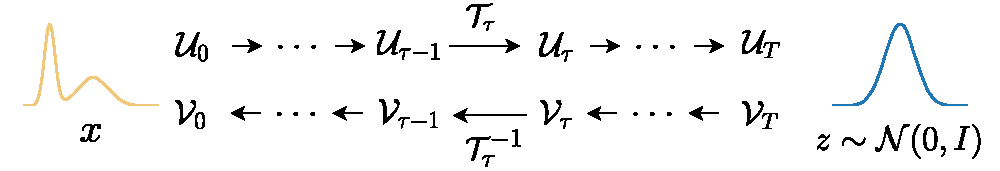
\includegraphics[width=0.85\textwidth]{figures/SNF.pdf}
    \caption[SNF Architecture]{The architecture of an \ac{SNF} with Markov chains $((U_0, \ldots, U_T), (V_T, \ldots, V_0))$. $T$ is the number of stochastic blocks. We denote the transformation in the forward process (from data to latent) by $\textcolor{NavyBlue}{\mathcal{T}_t = P_{U_t \mid U_{t-1}}}$ and that in the inverse process (from latent to data space) by $\textcolor{Orange}{\mathcal{T}_t^{-1} = P_{V_{t-1} \mid V_t}}$. To be consistent with \ac{NF} as shown in Figure~\ref{fig:bayesflow}, the left side of the figure is the data distribution, while the right side is the latent distribution. Usually, the latent variable follows a standard normal distribution. The upper row illustrates the forward direction from data to latent space, whereas the bottom row shows the inverse direction from latent to data space.}
    \label{fig:snf}
\end{figure}

Unlike \acp{CNF}, for which the objective function is minimizing the KL-divergence between the learned and target density, the objective function for training an \ac{SNF} is to minimize the difference of the joint distributions between the forward and inverse processes. We define the joint distributions as:
\begin{subequations}
\begin{align}
    \textcolor{NavyBlue}{P_{U_{0:T}}} &= \textcolor{NavyBlue}{P_{U_0\sim p_X}\prod_{t=1}^{T}P_{U_{t}|U_{t-1}}} && \text{(forward: data $\to$ latent)}, \\
    \textcolor{Orange}{P_{V_{0:T}}} &= \textcolor{Orange}{P_{V_T\sim p_Z}\prod_{t=1}^{T}P_{V_{t-1}|V_t}} && \text{(inverse: latent $\to$ data)}.
\end{align}
\end{subequations}
Then, the objective taking the forward process as training variables is:
\begin{equation}
    \mathcal{L}_{SNF}(\theta)=D_{\text{KL}}(\textcolor{Orange}{P_{V_{0:T}}}||\textcolor{NavyBlue}{P_{U_{0:T}}})=\mathbb{E}_{u_{0:T}\sim P_{V_{0:T}}}\log \frac{d\textcolor{Orange}{P_{V_{0:T}}}}{d\textcolor{NavyBlue}{P_{U_{0:T}}}}.
\end{equation}
Similar to \acp{CNF}, the objective function of an \ac{SNF} is trained from data to the latent space. The derivative term can be expanded as:
\begin{equation}
    \frac{d\textcolor{Orange}{P_{V_{0:T}}}}{d\textcolor{NavyBlue}{P_{U_{0:T}}}} = \frac{\textcolor{Orange}{p_{V_0}(u_0)}}{\textcolor{NavyBlue}{p_{U_0}(u_0)}}\prod_{t=1}^{T}\frac{\textcolor{Orange}{p_{V_t|V_{t-1}}(u_t|u_{t-1})}}{\textcolor{NavyBlue}{p_{U_t|U_{t-1}}(u_t|u_{t-1})}}=\frac{\textcolor{Orange}{p_{V_T}(u_T)}}{\textcolor{NavyBlue}{p_{U_T}(u_T)}}\prod_{t=1}^{T}\frac{\textcolor{Orange}{p_{V_{t-1}|V_t}(u_{t-1}|u_t)}}{\textcolor{NavyBlue}{p_{U_{t-1}|U_t}(u_{t-1}|u_t)}}.
\end{equation}
Because $V_T\equiv Z$ and $U_0\equiv X$ and the SNF is trained from $U_0$ to $U_T$, the term can be rewritten as:
\begin{equation}
    \frac{d\textcolor{Orange}{P_{V_{0:T}}}}{d\textcolor{NavyBlue}{P_{U_{0:T}}}} = \frac{\textcolor{Orange}{p_{V_T}(u_T)}}{\textcolor{NavyBlue}{p_{U_0}(u_0)}}\prod_{t=1}^{T}\textcolor{RoyalPurple}{f_t(u_{t-1}, u_t)}\frac{\textcolor{Orange}{p_{V_{t-1}}(u_{t-1})}}{\textcolor{Orange}{p_{V_t}(u_t)}}, \quad \textcolor{RoyalPurple}{f_t(u_{t-1}, u_t)}=\frac{\textcolor{Orange}{p_{V_t|V_{t-1}}(u_t|u_{t-1})}}{\textcolor{NavyBlue}{p_{U_t|U_{t-1}}(u_t|u_{t-1})}}.
\end{equation}
Then, the objective is:
\begin{equation}
    \mathcal{L}_{SNF}(\theta) = \mathbb{E}_{u_{0:T}\sim P_{V_{0:T}}}\left[\log \textcolor{Orange}{p_{V_T}(u_T)} - \log \textcolor{NavyBlue}{p_{U_0}(u_0)} + \sum_{t=1}^{T} \log \textcolor{RoyalPurple}{f_t(u_{t-1}, u_t)}\frac{\textcolor{Orange}{p_{V_{t-1}}(u_{t-1})}}{\textcolor{Orange}{p_{V_t}(u_t)}}\right]
\end{equation}
The term $\textcolor{RoyalPurple}{f_t(u_{t-1}, u_t)}p_{V_{t-1}}(u_{t-1})/p_{V_t}(u_t)\overset{\underset{\mathrm{def}}{}}{=}\textcolor{Magenta}{r}$ differs for deterministic and stochastic layers. For a \textbf{deterministic} transformation, $\textcolor{RoyalPurple}{f_t(u_{t-1}, u_t)=1}$ and $p_{V_{t-1}}(u_{t-1})/p_{V_t}(u_t)$ equals the change of variable:
\begin{equation}
    \textcolor{Magenta}{r} = \textcolor{RoyalPurple}{1}\cdot \frac{p_{V_{t-1}}(u_{t-1})}{p_{V_t}(u_t)} = \det \left|J_{\mathcal{T}_t}(u_{t-1})\right|.
\end{equation}
For a \textbf{stochastic} transformation, $\textcolor{Magenta}{r}$ measures how well the backward kernel inverts the forward one; it can be reformulated as:
\begin{equation}
    \textcolor{Magenta}{r} = \frac{\textcolor{Orange}{p_{V_t|V_{t-1}}(u_t|u_{t-1})}}{\textcolor{NavyBlue}{p_{U_t|U_{t-1}}(u_t|u_{t-1})}}\frac{\textcolor{Orange}{p_{V_{t-1}}(u_{t-1})}}{\textcolor{Orange}{p_{V_t}(u_t)}} = \frac{\textcolor{Orange}{p_{V_{t-1}|V_t}(u_{t-1}|u_t)}}{\textcolor{NavyBlue}{p_{U_t|U_{t-1}}(u_t|u_{t-1})}}.
\end{equation}
The stochastic layer must be invertible and fulfill the detailed balance condition for some density $\textcolor{OliveGreen}{\pi_t}$:
\begin{equation}
    \label{eq:det_bal}
    \textcolor{OliveGreen}{\pi_t(u_t)}\textcolor{Orange}{p_{V_{t-1}|V_t}(u_{t-1}|u_t)} = \textcolor{OliveGreen}{\pi_{t}(u_{t-1})}\textcolor{NavyBlue}{p_{U_t|U_{t-1}}(u_t|u_{t-1})}.
\end{equation}
where $\textcolor{OliveGreen}{\pi_t}$ is the target density at step $t$, interpolating between $p_Z$ and $p_X$: $\textcolor{OliveGreen}{\pi_t} = c \cdot p_Z^{t/T} \cdot p_X^{(T-t)/T}$ with $c$ a normalizing constant and $E_t(u)=-\log(\textcolor{OliveGreen}{\pi_t(u)})$. Rearranging Equation~\ref{eq:det_bal}:
\begin{equation}
    \textcolor{Magenta}{r}=\frac{\textcolor{Orange}{p_{V_{t-1}|V_t}(u_{t-1}|u_t)}}{\textcolor{NavyBlue}{p_{U_t|U_{t-1}}(u_t|u_{t-1})}}=  \frac{\textcolor{OliveGreen}{\pi_t(u_{t-1})}}{\textcolor{OliveGreen}{\pi_t(u_{t})}}.
\end{equation}
For \ac{MCMC} this is computed by evaluating $\textcolor{OliveGreen}{\pi_t}$; for efficiency an \ac{MALA} kernel (Section~\ref{sec:MALA}) yields:
\begin{equation}
    \textcolor{Magenta}{r} = \frac{\textcolor{OliveGreen}{\pi_t(u_{t-1})}}{\textcolor{OliveGreen}{\pi_t(u_{t})}} = \exp\left(\frac{1}{2}\left(\left\|\textcolor{Orange}{\tilde{\eta}_t}\right\|^2_2-\left\|\textcolor{NavyBlue}{\eta_t}\right\|^2_2\right)\right),
\end{equation}
where the Gaussian noise vectors are:
\begin{align}
    \textcolor{NavyBlue}{\eta_t} &:= \frac{1}{\sqrt{\tau}} \left( u_{t-1} - u_t - \frac{\tau}{2} \nabla E_t(u_{t-1}) \right) && \text{(forward: } u_{t-1}\to u_{t}\text{)}, \\
    \textcolor{Orange}{\tilde{\eta}_t} &:= \frac{1}{\sqrt{\tau}} \left( u_{t-1} - u_t + \frac{\tau}{2} \nabla E_t(u_t) \right) && \text{(backward: } u_{t}\to u_{t-1}\text{)}.
\end{align}

\subsubsection{Experiments on Stochastic Normalizing Flows}
We evaluate \acp{SNF} on two fronts: multimodal posterior modeling and parameter identification under noisy observations. The following experiments demonstrate the practical benefits of combining normalizing flows with stochastic \ac{MCMC} layers.

\begin{figure}[ht]
    \centering
    \begin{minipage}[t]{0.55\textwidth}
        % \setlength{\abovecaptionskip}{0pt} 
        \vspace{0pt}
        \captionof{figure}[Multimodal Modeling Comparison between NF and SNF]{Comparison of MCMC-RealNVP (left) and RealNVP (right) for multimodal modeling. Experimental settings match Fig.~\ref{fig:mm_comp}.}
        \label{fig:snf_mm}
        \vspace{3.5em}
        \captionof{table}[Multimodal Modeling Comparison]{Comparison of Posterior Estimation Metrics. For RMSE/MCIW, lower is better ($\downarrow$); for CICP, $\approx 0.95$ is ideal. Metrics are mode-aligned with centers identified via $K$-means clustering. The results except the MCMC are corresponding to Figure \ref{fig:mm_comp}. The MCMC stands for an SNF with MCMC and RealNVP. }
        \label{tab:mm_comparison}
        \vspace{0.5em}
        \centering
        \small
        \begin{tabular}{l ccc}
            \toprule
            \textbf{Model} & \textbf{RMSE} ($\downarrow$) & \textbf{MCIW} ($\downarrow$) & \textbf{CICP} \\
            \midrule
            BNN     & 1.611 & 4.581 & 0.843 \\
            VAE     & 1.375 & 1.527 & 0.460 \\
            DDPM    & 1.415 & 2.211 & 0.560 \\
            SBM     & 0.540 & 0.838 & 0.553 \\
            FM      & 0.300 & 0.830 & 0.873 \\
            RealNVP & 0.258 & 1.067 & 0.925 \\
            NSF     & 0.108 & \textbf{0.412} & 0.928 \\
            MCMC   & \textbf{0.105} & 0.508 & \textbf{0.970} \\
            \bottomrule
        \end{tabular}

    \end{minipage}
    \hfill
    \begin{minipage}[t]{0.43\textwidth}
        \centering
        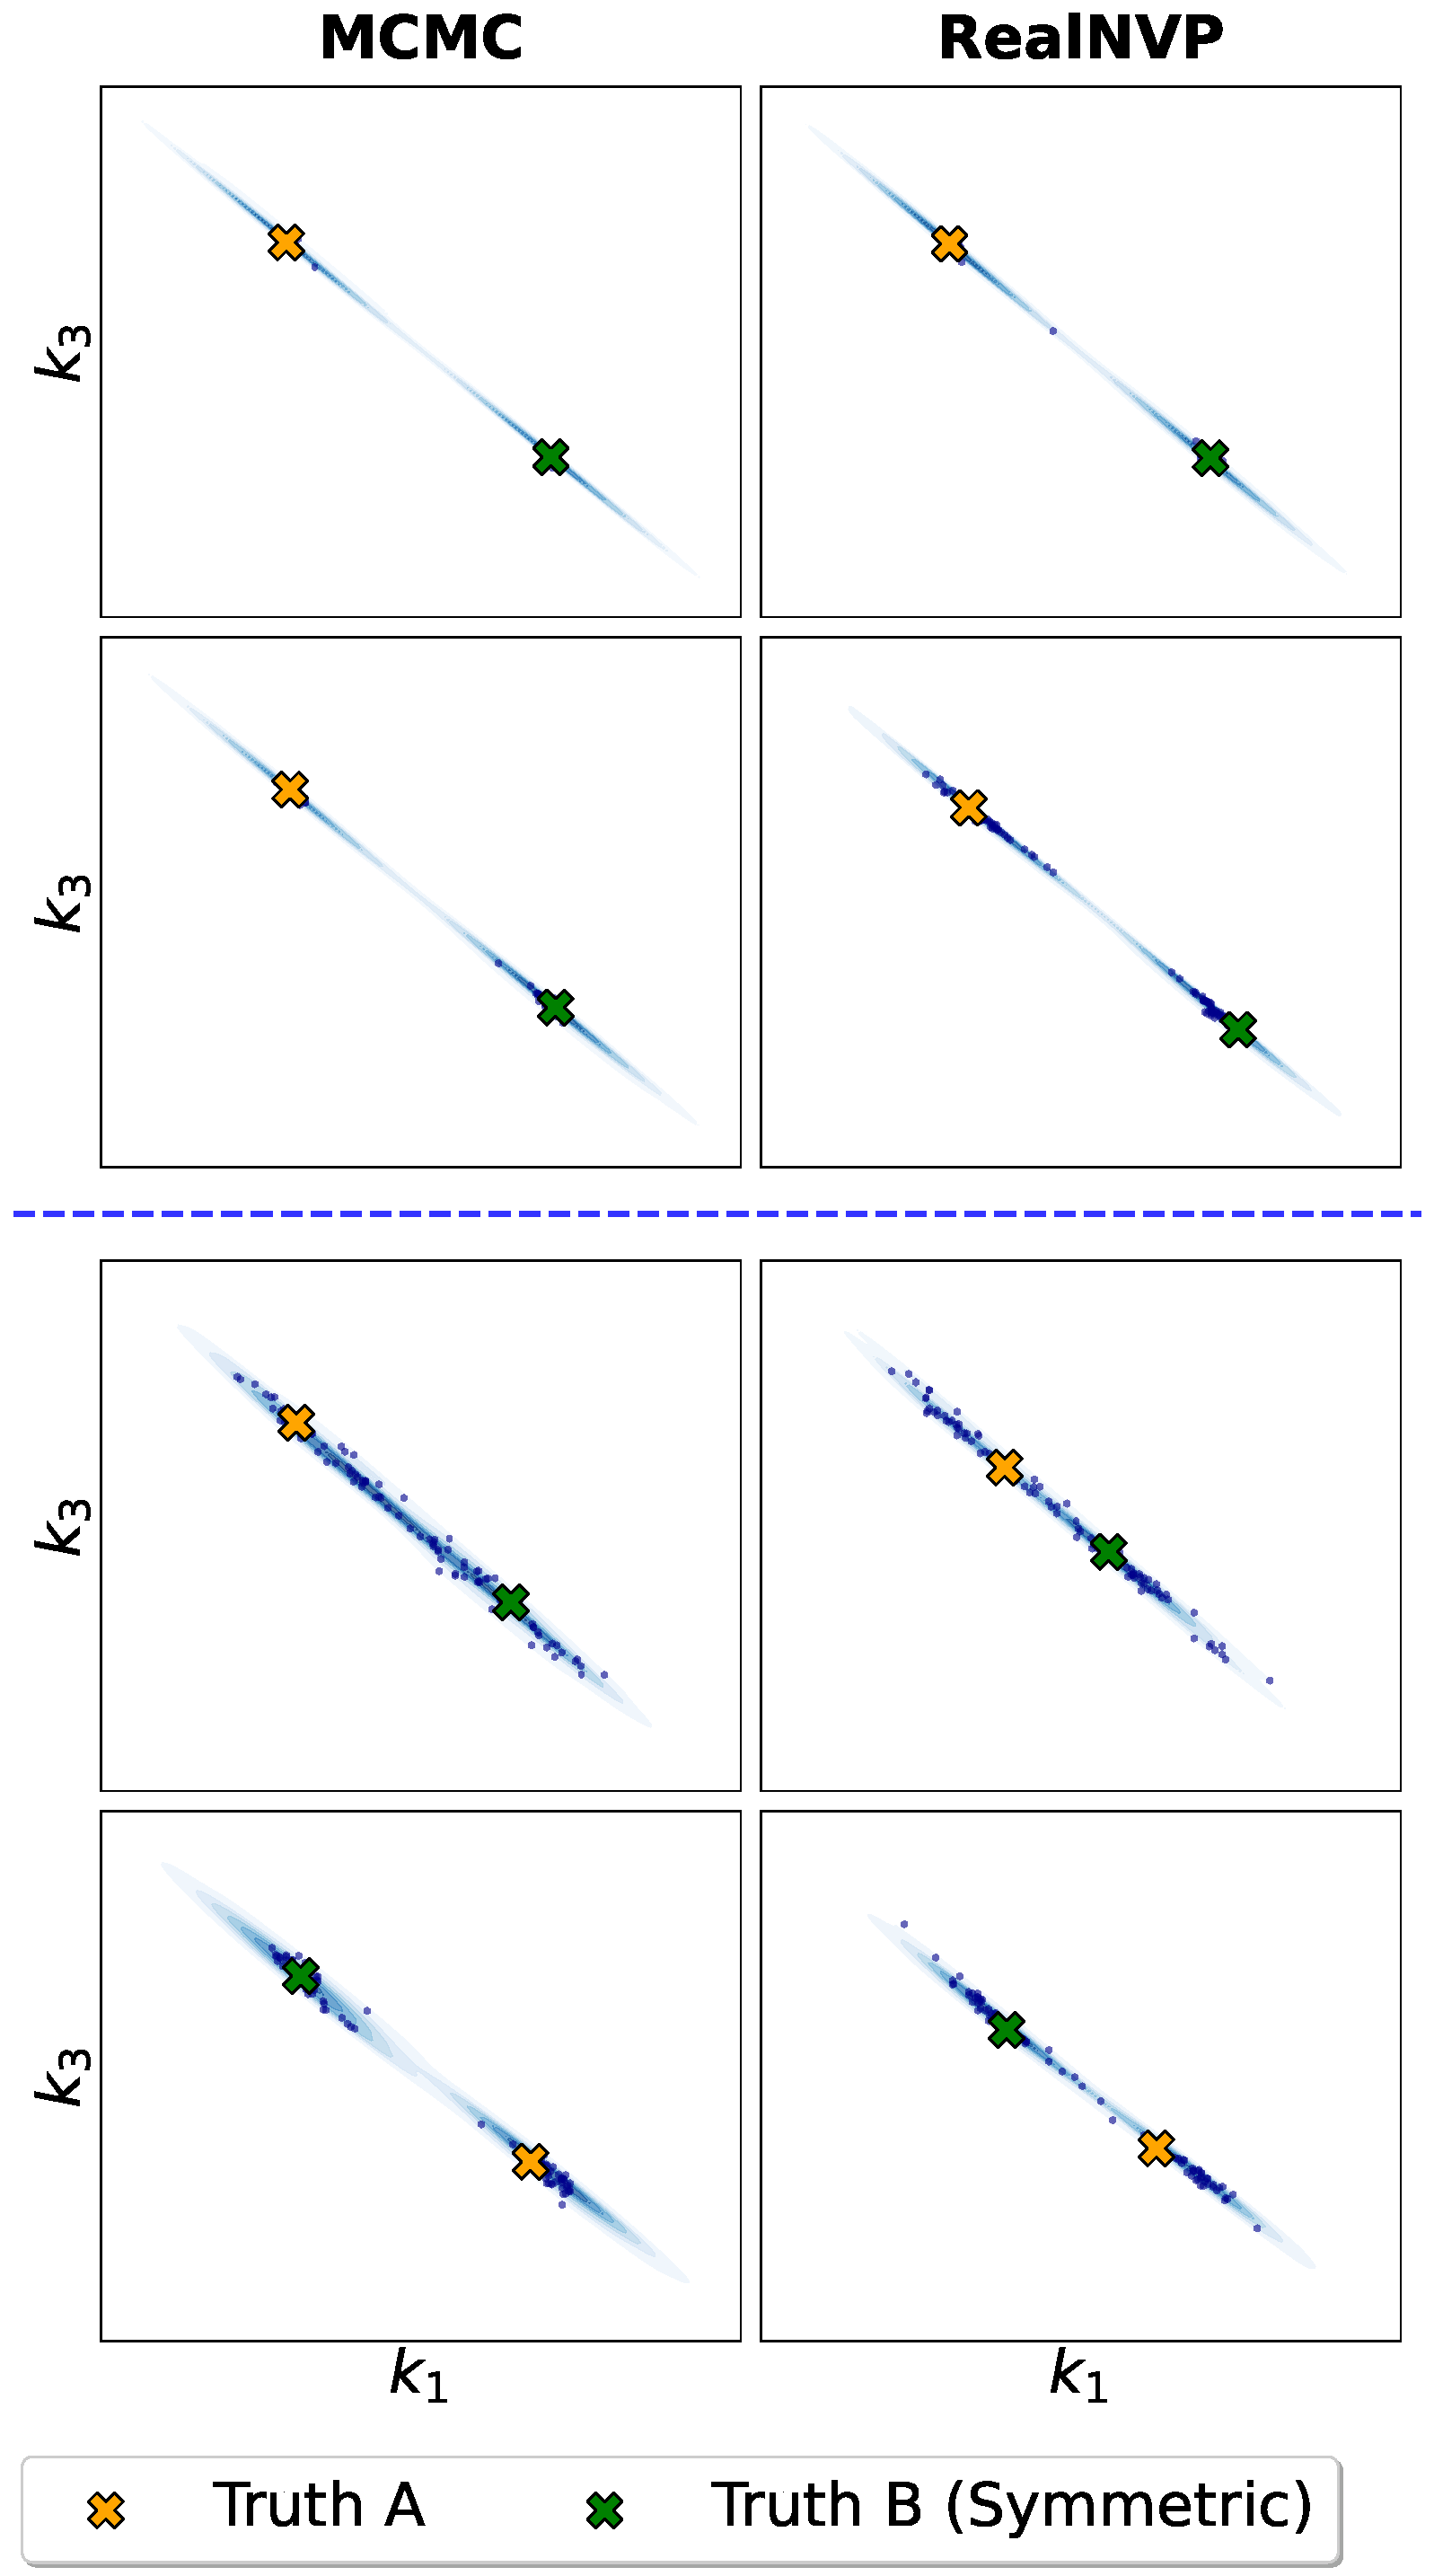
\includegraphics[width=\textwidth, valign=T]{figures/model_comparison_grid_multi_modal_snf.pdf}
    \end{minipage}
\end{figure}
To enhance multimodal modeling, we implement a hybrid \ac{SNF} architecture combining \ac{RealNVP} with four intermediate \ac{MCMC} refinement steps (step size is 0.001). In the forward (training) pass, the \ac{MCMC} updates are applied to the latent encoding to improve likelihood estimation; in the inverse (generative) pass, they are applied to the output samples to ensure better alignment with the target data distribution. This stochastic refinement enables the flow to capture disconnected modes, which are challenging for \ac{RealNVP} as a simpler deterministic \ac{NF}. Table \ref{tab:mm_comparison} demonstrates that this approach yields the best-in-class RMSE and a near-ideal coverage probability, outperforming the \ac{NSF} (top performer in our study) in terms of both precision and uncertainty quantification.

In order to improve the parameter identifiability under noisy observations, we apply a \ac{MALA}-refinement after sampling through \ac{NF} architecture. We define the log-likelihood by measuring the residual between the actual observations and the signals generated by the model's governing dynamics using the inferred parameters. For the sake of handling different parameter sensitivity, the \ac{RMALA} refinement leverages the Fisher Information Matrix (or Hessian) to adapt to the local curvature of the log-posterior. While standard \ac{MALA} uses a constant step size in all directions, \ac{RMALA} uses a position-dependent metric tensor. This preconditioning allows the flow to take larger steps in directions of low sensitivity and smaller, more precise steps in directions of high sensitivity.

\begin{figure}[H]
    \centering
    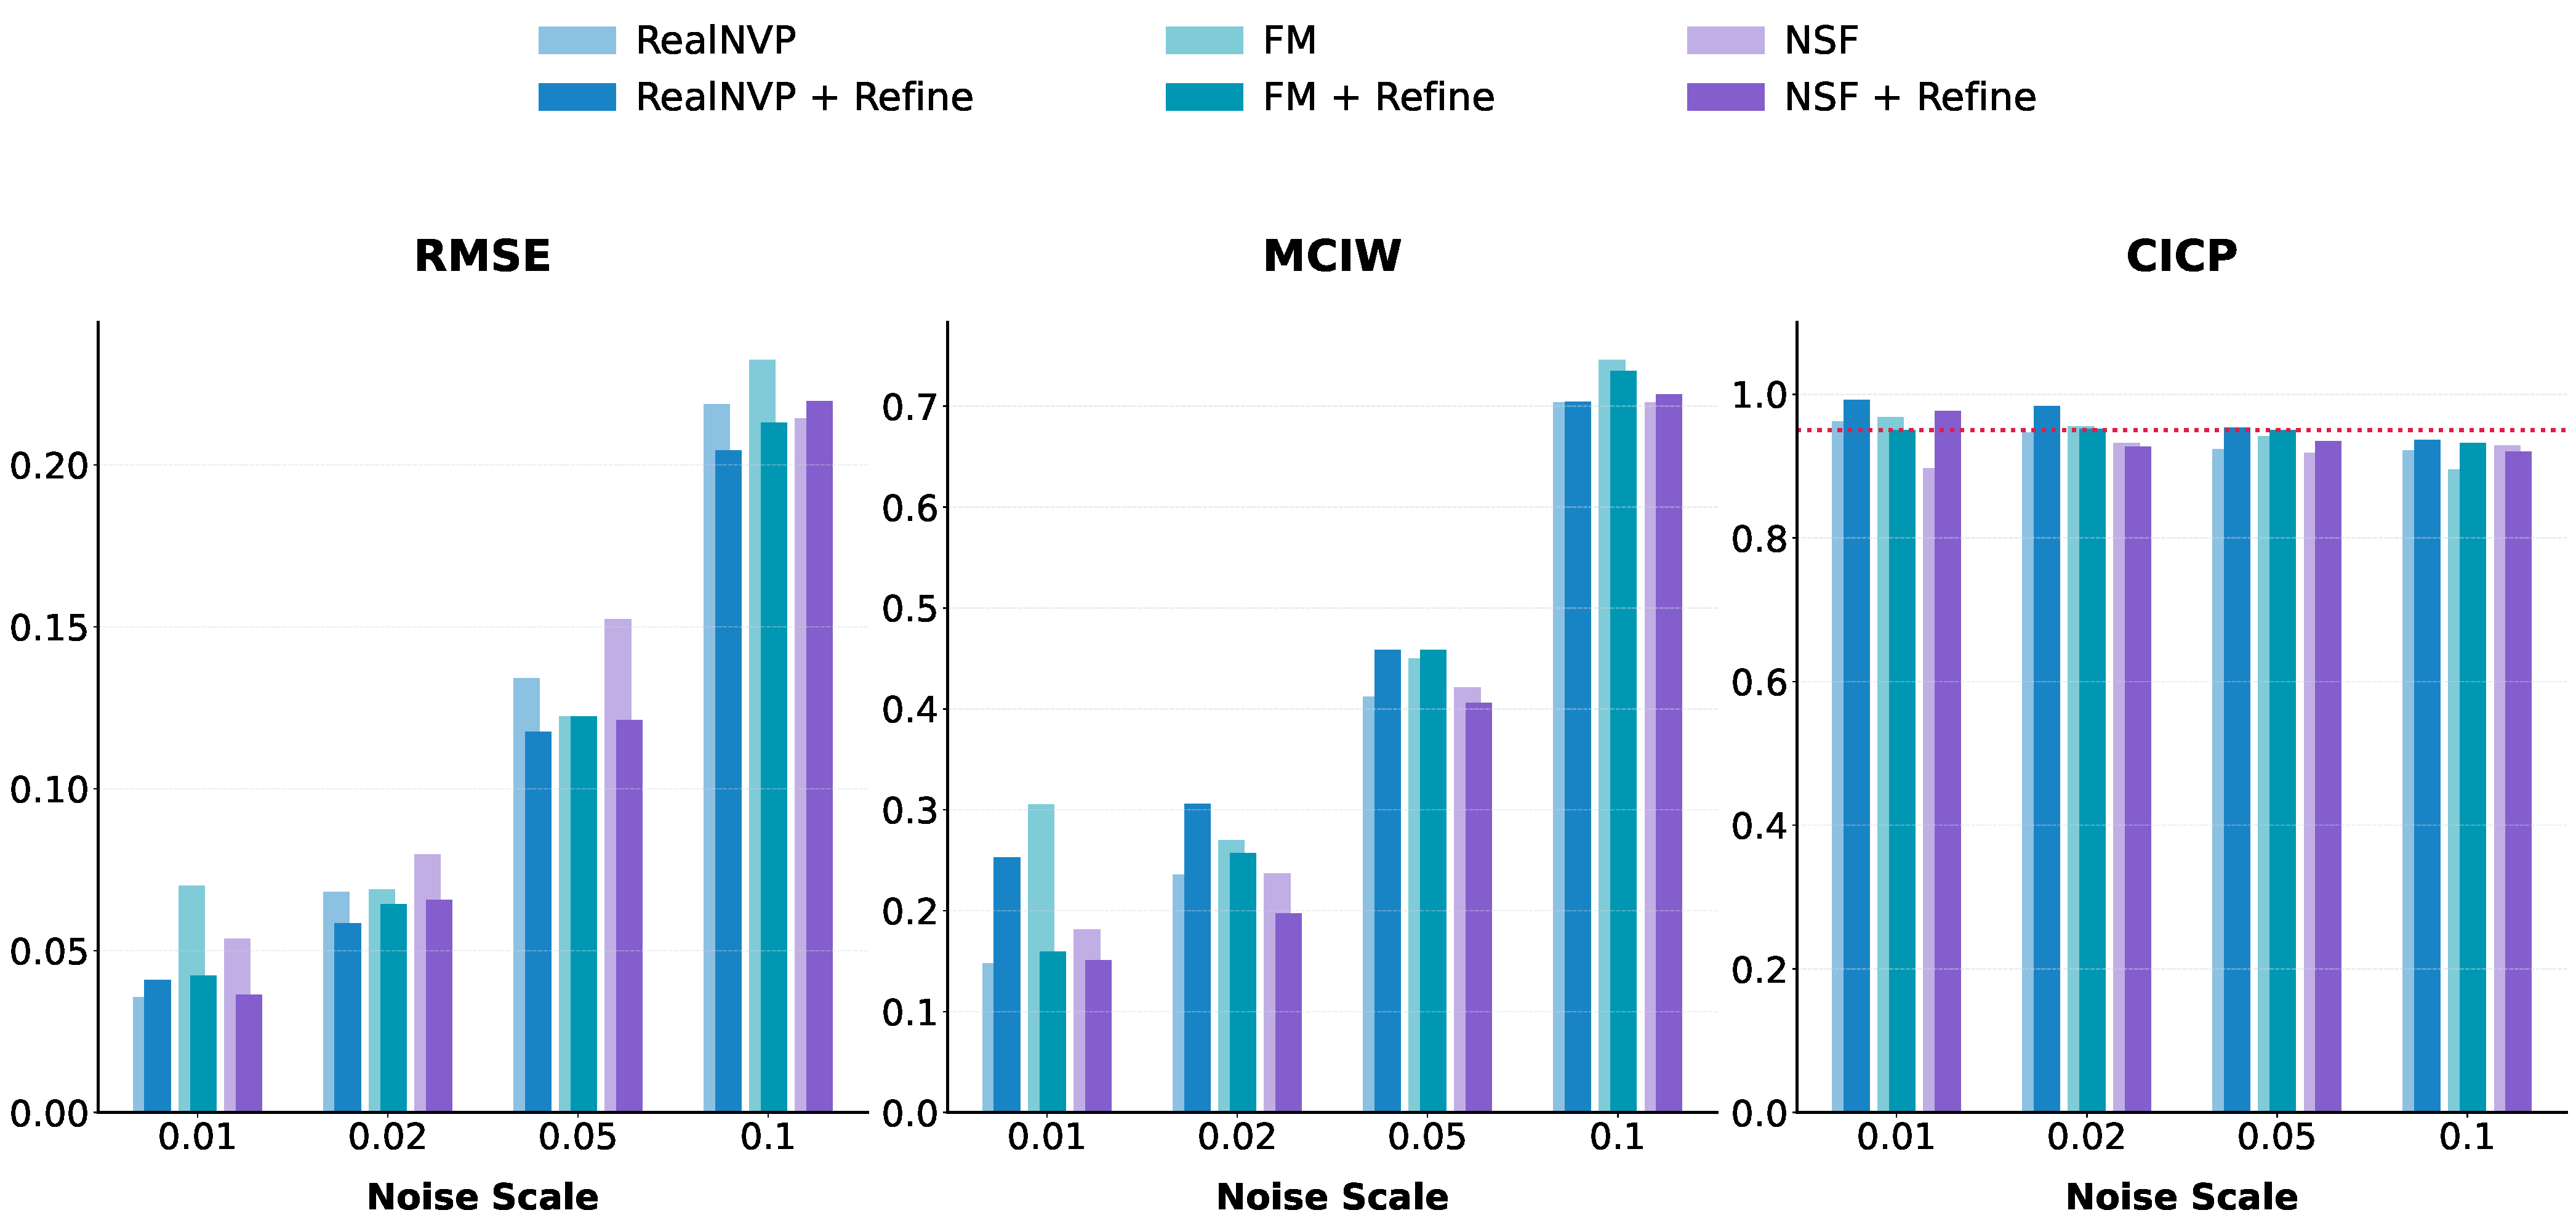
\includegraphics[width=\textwidth]{figures/snf_refine_comparison.pdf}
    \caption[Improved Parameter Identification Under Noisy Observations with SNF]{Improved Parameter Identification under Noisy Observations using \acp{SNF}. Three \ac{NF} architectures—\ac{RealNVP}, \ac{FM}, and \ac{NSF}—are evaluated across varying noise scales (0.01, 0.02, 0.05, and 0.1). Performance is measured in terms of accuracy (RMSE) and uncertainty quantification (MCIW and CICP). Grouped bars contrast the original baseline results with those obtained via \ac{RMALA}-based refinement. In the CICP subfigure, the dashed red line indicates the ideal coverage probability of 0.95.}
    \label{fig:snf_refinement}
\end{figure}

Figure \ref{fig:snf_refinement} shows the comparison of parameter identification under noisy observations between \ac{NF} and \ac{SNF}. The RMSE panel reveals a clear trend where error increases proportionally with observational noise. However, the stochastic refinement consistently outperforms the deterministic base models across all noise scales. At lower noise levels (0.01 and 0.02), the refined models often exhibit a higher MCIW than the base models. It indicates that the base models were producing intervals that were too narrow (overconfident). The \ac{MALA} layers broaden the distribution to accurately reflect the true posterior width. At a noise scale of 0.1, the MCIW values converge. This suggests that in high-noise regimes, the scale of uncertainty is largely driven by the data likelihood rather than the specific choice of flow architecture. The uncertainty calibration can be proven in the CICP panel as well. Note that at noise scale 0.01, the base \ac{NSF} model (light purple) significantly under-0.95-covers. The refinement step (dark purple) lifts this probability back to the target. While deterministic models start to lose coverage as noise increases (falling below 0.90), the refined models maintain a much more stable coverage probability, remaining close to the target across the entire noise spectrum. The consistent improvement in CICP implies that the stochastic layers are pushing the approximate posterior much closer to the true posterior. 

Surprisingly, the \ac{FM} reaches exact 0.95 CICP at noise scales (0.01, 0.02 and 0.05). Because \ac{FM} learns a continuous vector field rather than a series of discrete couplings, it likely provides a smoother initial density for the stochastic layers. When \ac{RMALA} is applied to this smooth surface, the gradient-based steps can move the samples to the exact posterior boundaries with higher precision than in more rigid architectures like \ac{RealNVP} and \ac{NSF}. This makes the \ac{RMALA}-refined \ac{FM} an exceptionally reliable tool for parameter identification in complex, noisy dynamical systems.
 
